\documentclass[11pt]{article}
\usepackage[utf8]{inputenc}
\usepackage{amsmath} % For mathematical symbols
\usepackage{amssymb}
\usepackage{graphicx} % To include figures
\usepackage[margin=0.5in]{geometry} % To set margins
\usepackage{cite}
\usepackage{enumitem}
\usepackage{algorithm}
\usepackage{xcolor}
\usepackage{booktabs}
\usepackage{listings}
\usepackage{url}
\usepackage{algpseudocode}
\usepackage{tikz}
\usetikzlibrary{positioning}   % for "right=of", "below=of" syntax
\usetikzlibrary{arrows.meta}   % for >=stealth arrow style

% Custom commands
\newcommand{\R}{\mathbb{R}}
\newcommand{\Cfree}{\mathcal{C}_{\text{free}}}
\newcommand{\Cobs}{\mathcal{C}_{\text{obs}}}
\newcommand{\C}{\mathcal{C}}
\newcommand{\T}{\mathcal{T}}
\newcommand{\vnear}{v_{\text{near}}}
\newcommand{\vnearest}{v_{\text{nearest}}}
\newcommand{\vinit}{v_{\text{init}}}
\newcommand{\xrand}{x_{\text{rand}}}
\newcommand{\xnew}{x_{\text{new}}}
\newcommand{\xinit}{x_{\text{init}}}
\newcommand{\xgoal}{x_{\text{goal}}}

\newtheorem{theorem}{Theorem}
\newtheorem{proposition}{Proposition}
\newtheorem{lemma}{Lemma}


\title{Autonomous Robot Exploration using Landmark-based EKF-SLAM}

\author{
	Piyush Bhansali \\
	\textit{Department of Industrial Engineering} \\
	\textbf{University of Trento} \\[2ex]
	Supervised by: \\
	Professor Daniele Fontanelli
}

\date{\today}

\begin{document}
	
	\maketitle
	\vspace{1em}
	
	% --- ABSTRACT (Unchanged to keep your specific abstract style) ---
	\begin{abstract}
		\bfseries
		\noindent
		Autonomous exploration and mapping of unknown environments remain a fundamental challenge in mobile robotics, with applications spanning search and rescue operations, warehouse automation, planetary exploration, and autonomous navigation. This thesis develops and evaluates a feature-based SLAM system for autonomous indoor navigation on TurtleBot3 Waffle Pi robot.
		
		\vspace{0.5em}
		\noindent
		The system uses a 360° 2D LiDAR as its primary sensor. Raw range scans are processed to extract geometric landmarks like walls and corners. Walls are parameterised in Hessian normal form $(\rho, \alpha)$, and corners are stored using the cartesian coordinates $(x, y)$. Wall segments are extracted using the Incremental line fitting and merge algorithm and corners are extractde by determining the intersection points between two adjacent walls.
		
		\vspace{0.5em}
		\noindent
		While Feature based SLAM methods have been extensively studied, probabilistic mapping that explicitly captures landmark uncertainty and its correlation with the robot—especially when using point‑cloud data—remains limited. This thesis addresses that gap by computing wall covariances via the Cramér–Rao lower bound and corner covariances via error propagation through line‑intersection geometry, making uncertainty quantification a primary research objective. Map confidence is thus defined directly by these covariances, and the probabilistic estimation of both landmarks and the robot becomes the central focus of the work.
			 	
		\vspace{0.5em}
		\noindent
		State estimation is performed by an Extended Kalman Filter (EKF). The state vector contains the robot pose $(x, y, \theta)$ and all landmark parameters jointly, so that a single observation updates both the observed landmark and every other landmark through the cross-covariance structure. Landmarks are matched to observations using nearest-neighbour association with Mahalanobis-distance gating at the 95\% chi-squared confidence level. Global consistency is maintained by a submap-stitching layer that uses feature-based SVD alignment. This correction is injected into the EKF as a direct pose observation, propagating the adjustment to all correlated landmarks through the cross-covariance structure.
		
		
		\vspace{0.5em}
		\noindent
		The navigation module enables autonomous exploration through frontier
		detection and path planning. Frontiers are identified by computing the
		convex hull of known map and sampling the boundary as potential
		exploration goals. The RRT* algorithm plans collision-free paths to
		selected frontiers, whereas a pure pursuit controller tracks the planned paths.
		
		\vspace{0.5em}
		\noindent
		The system is implemented as a ROS 2 node in Python, tested on TurtleBot3 in structured indoor environments. Performance is assessed using the absolute trajectory error (ATE), landmark map confidence, point cloud quality, and filter consistency via the normalised estimation error squared (NEES).
				
			
		\vspace{0.5em}
		\noindent
		Keywords: SLAM, Extended Kalman Filter, Feature-Based Mapping, Landmark Extraction, SVD Alignment, Procrustes, RRT*, ROS2, Frontier-Based Exploration, 2D LiDAR Mapping, Cramér-Rao Lower Bound
	\end{abstract}
	
	\newpage
	\tableofcontents
	\newpage
	
	% --- GLOBAL PARAGRAPH FORMATTING CHANGE ---
	\setlength{\parindent}{0pt} % Remove indentation for all paragraphs
	\setlength{\parskip}{0.5em} % Add vertical space between all paragraphs
	\pagebreak
	% --- INTRODUCTION ---
	\section{Introduction}
	
	\subsection{Motivation}
	
	\subsubsection{The need for Autonomous Exploration}
	
	The ability of mobile robots to autonomously explore and map unknown environments is one of the most fundamental challenges in robotics. Unlike structured industrial settings where environments are precisely, many real-world scenarios require robots to operate in previously unmapped, and potentially hazardous spaces where human presence is dangerous or impossible. This necessity drives the application of autonomous exploration across several critical domains such as Search and Rescue Operations, Warehouse and Logistics Automation, Planetary and Underground Exploration etc. While teleoperated robots provide an alternative to direct human presence, it requires  high bandwidth, low-latency communication channels and are prone to human errors. Furthermore, operational costs scale linearly with the number of robots, making large-scale swarm management unsustainable.
	
	\subsubsection{The SLAM Problem: Fundamental Challenge of Robotics} 

	One of the critical challenges faced in autonomous exploration is the Simultaneous Localization and Mapping (SLAM) problem \cite{durrant2006slam}: an algorithm to build a map of an unknown environment while simultaneously using that map to determine its own location, creating a circular dependency often described as a "chicken-and-egg" problem. 
	
 	One of the methods is to compute the posterior distribution of the robot state and map given all sensor measurements and control inputs over time. \cite{thrun2005probabilistic}. Smith and Cheeseman (1987) formalised the problem using covariance matrices to represent spatial uncertainty. Dissanayake et al. (2001) provided the first convergence proof for SLAM. They showed that the determinant of any submatrix of the landmark covariance decreases monotonically as observations accumulate, meaning the map becomes more certain over time\cite{Dissanayake2001}.
	
	Indoor environments are dominated by planar surfaces, making lines and corners superior landmarks compared to raw points or occupancy grids. The task of converting raw 2D range data into these landmarks is a well-studied problem. Nguyen et al. (2005) \cite{Nguyen} conducted a comparative analysis of four feature extraction methodologies: Split-and-Merge, Incremental Line Fitting, the Hough Transform, and RANSAC. While the Hough Transform and RANSAC are known for their robustness to outliers, they often come with a higher computational cost whereas Split-and-Merge and Incremental Line Fitting provide the best balance of reliability and speed. Given that LiDAR sensors provide ordered scans, the Incremental Line Fitting method was selected for this work.
 	
	Feature based EKF-SLAM represents the environment as a set of walls and corners, each with a covariance that describes how uncertain it is with respect to the robot. When a landmark is re-observed, the correction spreads coherently to every other correlated landmark through the joint covariance matrix.
	 

\subsection{Problem Statement}

One of the challenges faced in indoor SLAM, is unavailability of Global Navigation Satellite System (GNSS). The robot has to rely on noisy sensor data for localisation and mapping, which inherently couples the errors in robot pose estimation with the extracted environmental features. Many current feature-based methodologies utilize heuristic approximations for landmark uncertainty or fail to account for the correlations between the robot and the map. As a result, maps can appear geometrically plausible while being statistically overconfident, limiting their reliability for downstream navigation and evaluation.

This thesis addresses that gap by developing and assessing a feature‑based EKF‑SLAM system with explicit uncertainty modeling for both walls and corners. Wall covariances are derived from the Fisher information (Cramér–Rao lower bound) of the line fit, and corner covariances are propagated analytically through the line‑intersection geometry, yielding a principled measure of map confidence. The objective is to quantify and preserve probabilistic map quality while evaluating localization accuracy, landmark consistency, and overall mapping performance in indoor environments.

\subsection{Autonomous Exploration and Navigation}

Frontier-based exploration identifies the boundary between mapped free space and unknown territory as navigation goals. In contrast to classic grid‑based frontier exploration\cite{Yamauchi1997}, a point‑cloud frontier strategy operates directly on lidar returns without discretizing space. The approach used in this thesis is to compute the convex hull of the observed free points and treat the hull boundary as a frontier surface; multiple candidates are then selected based on reachability, travel cost, and expected information gain. 

\textit{RRT*} algorithm \cite{karaman2011sampling}, which offers asymptotic optimality is used for higher level path planning. For path tracking, the \textit{Pure Pursuit} controller \cite{coulter1992} is selected for its simplicity and smooth steering behavior, using a lookahead distance calibrated for the differential-drive kinematics of the TurtleBot3.


\subsection{Thesis Contributions}

While landmark based EKF-SLAM and frontier exploration have been studied extensively, probabilistic based mapping using geometry-aware CRLB covariances for landmarks and feature-based SVD drift correction is the objective of this thesis. A convex‑hull–based frontier detection algorithm which operates directly on the point cloud to generate exploration targets without grid discretization is implemented, where frontier candidates are geometrically validated and ranked for navigation.

A core contribution of this work is also the explicit modeling of landmark uncertainty within the EKF state vector. Rather than treating landmarks as isolated points, the system maintains a joint covariance matrix that captures the high degree of correlation between the robot’s pose and the mapped features. Furthermore, this framework provides a confidence metric by aggregating the marginal uncertainties of the landmarks associated with a specific submap.

\section{THEORY}

\subsection{SLAM Problem Statement}

The simultaneous localization and mapping problem can be formally stated as follows. Let $\mathbf{x}_t = [x_t, y_t, \theta_t]^T \in \mathbb{SE}(2)$ represent the robot's pose at time $t$ in the special Euclidean group, where $(x_t, y_t)$ denotes the position in Cartesian coordinates and $\theta_t$ denotes the orientation. Let $\mathcal{M} = \{\mathbf{p}_i\}_{i=1}^{N}$ represent the map as a set of $N$ points in $\mathbb{R}^2$, where each $\mathbf{p}_i = [p_i^x, p_i^y]^T$ represents a landmark or environment feature.

At each time step, the robot receives control inputs $\mathbf{u}_t = [v_x, v_y, \omega]^T$ representing linear velocities and angular velocity, and sensor observations $\mathbf{z}_t$ representing laser range measurements. The sequence of poses, control inputs, and observations up to time $t$ is denoted as:
\begin{align}
	\mathbf{X}_{0:t} &= \{\mathbf{x}_0, \mathbf{x}_1, \ldots, \mathbf{x}_t\} \\
	\mathbf{U}_{1:t} &= \{\mathbf{u}_1, \mathbf{u}_2, \ldots, \mathbf{u}_t\} \\
	\mathbf{Z}_{1:t} &= \{\mathbf{z}_1, \mathbf{z}_2, \ldots, \mathbf{z}_t\}
\end{align}

The full SLAM problem seeks to estimate the posterior distribution over all poses and the map given the observations and controls:
\begin{equation}
	p(\mathbf{X}_{0:t}, \mathcal{M} \mid \mathbf{Z}_{1:t}, \mathbf{U}_{1:t})
\end{equation}

However, computing this full joint posterior is computationally intractable for large-scale problems. Therefore, this implementation adopts an online filtering approach where we incrementally estimate the current pose and map, marginalizing out past poses:
\begin{equation}
	p(\mathbf{x}_t, \mathcal{M} \mid \mathbf{Z}_{1:t}, \mathbf{U}_{1:t})
\end{equation}

\subsubsection{Motion Model}

The robot's motion follows a discrete-time kinematic model with additive Gaussian noise. The state transition probability is given by:
\begin{equation}
	p(\mathbf{x}_t \mid \mathbf{x}_{t-1}, \mathbf{u}_t) = \mathcal{N}(\mathbf{x}_t; f(\mathbf{x}_{t-1}, \mathbf{u}_t), \mathbf{Q}_t)
\end{equation}

where $f(\cdot)$ is the deterministic motion function and $\mathbf{Q}_t$ is the process noise covariance matrix. For a differential-drive robot, the motion function in the global frame is:

\[
f(\mathbf{x}_{t-1}, \mathbf{u}_t) 
=
\begin{bmatrix}
	x_{t-1} + \delta_d \cos(\theta_{t-1} + \delta_\theta / 2) \\
	y_{t-1}  + \delta_d \sin(\theta_{t-1} + \delta_\theta / 2) \\
	\theta_{t-1} + \delta_\theta
\end{bmatrix}
\]

The process noise covariance $\mathbf{Q}_t$ accounts for unmodeled dynamics, wheel slippage, and discretization errors. It is parameterized as a diagonal matrix:
\begin{equation}
	\mathbf{Q}_t = \begin{bmatrix}
		\sigma_d^2 & 0 \\
		0 & \sigma_\theta^2\\
	\end{bmatrix}
\end{equation}

\subsubsection{Observation Model}

The laser range finder provides distance measurements to obstacles in the environment. For a 2D LiDAR with 360 beams, each observation $\mathbf{z}_t$ consists of 360 range-bearing pairs:
\begin{equation}
	\mathbf{z}_t = \{(r_j, \phi_j)\}_{j=1}^{M}
\end{equation}

where $r_j$ is the measured range and $\phi_j$ is the bearing angle relative to the sensor frame. These measurements are converted to Cartesian coordinates in the sensor frame:
\begin{equation}
	\mathbf{p}_j^{sensor} = \begin{bmatrix}
		r_j \cos(\phi_j) \\
		r_j \sin(\phi_j)
	\end{bmatrix}
\end{equation}

\subsection{Point Clouds}
A point Cloud is a set of data points containing coordinates that make up an object or an environment. They are primarily generated through exteroceptive sensors like LIDAR sensors and RGB-D Cameras. 

\subparagraph{LIDAR Point Cloud:} It is created by a LIDAR (Light Detection And Ranging) sensor, which emits thousands of laser pulses per second in all direction, and measures the relative position of an object depending on the time it takes the pulse to reflect off the surface and return to the sensor.

A LiDAR point cloud contains errors introduced from sensor-inherent, environmental, and geometric sources. These are mainly modelled as stochastic zero-mean gaussian noise.


\subsection{The Cramér–Rao Lower Bound (CRLB)}

The Cramér–Rao Lower Bound establishes a theoretical limit on the precision of an unbiased estimator. The CRLB is utilized to quantify the uncertainty of extracted geometric features, such as wall parameters $(\rho, \alpha)$ and SVD-based submap alignment results.

Let $\mathbf{\theta} \in \mathbb{R}^n$ represent an unknown parameter vector observed through a noisy measurement model:
\begin{equation}
	\mathbf{z} = h(\mathbf{\theta}) + \mathbf{v}, \quad \mathbf{v} \sim \mathcal{N}(\mathbf{0}, \mathbf{R}_{\text{sensor}})
\end{equation}

The covariance of any unbiased estimate $\mathbf{\hat{\theta}}$ is bounded by the inverse of the Fisher Information Matrix (FIM), denoted as $\mathcal{F}(\mathbf{\theta})$:
\begin{equation}
	\text{Cov}(\mathbf{\hat{\theta}}) \geq \mathcal{F}(\mathbf{\theta})^{-1}
\end{equation}

\subsection{Mahalanobis Distance}


The Mahalanobis distance is a measure of the distance between a point and a point or a point and a distribution. Unlike the Euclidean distance, which treats all dimensions equally, the Mahalanobis distance accounts for the correlations between variables. This makes it particularly useful in robotics and SLAM applications where sensor measurements have different uncertainties and may be correlated.

Given:
\begin{itemize}
	\item A point $\mathbf{x} \in \mathbb{R}^n$
	\item A distribution with mean $\boldsymbol{\mu} \in \mathbb{R}^n$
	\item Covariance matrix $\boldsymbol{\Sigma} \in \mathbb{R}^{n \times n}$ (positive definite)
\end{itemize}

The Mahalanobis distance from $\mathbf{x}$ to the distribution is:
\begin{equation}
	D_M(\mathbf{x}) = \sqrt{(\mathbf{x} - \boldsymbol{\mu})^T \boldsymbol{\Sigma}^{-1} (\mathbf{x} - \boldsymbol{\mu})}
\end{equation}

The squared Mahalanobis distance is:
\begin{equation}
	D_M^2(\mathbf{x}) = (\mathbf{x} - \boldsymbol{\mu})^T \boldsymbol{\Sigma}^{-1} (\mathbf{x} - \boldsymbol{\mu})
\end{equation}

\subparagraph{Distance Between Two Points}

For two points $\mathbf{x}, \mathbf{y} \in \mathbb{R}^n$ with covariance matrix $\boldsymbol{\Sigma}$:
\begin{equation}
	D_M(\mathbf{x}, \mathbf{y}) = \sqrt{(\mathbf{x} - \mathbf{y})^T \boldsymbol{\Sigma}^{-1} (\mathbf{x} - \mathbf{y})}
\end{equation}

\subsection{Singular Value Decomposition}

Compute the Single Value Decomposition of $\mathbf{H}$:
\begin{equation}
	\mathbf{H} = \mathbf{U}\mathbf{\Sigma}\mathbf{V}^T
\end{equation}

where:
\begin{itemize}
	\item $\mathbf{U} \in \mathbb{R}^{2 \times 2}$: orthogonal matrix (left singular vectors)
	\item $\mathbf{\Sigma} \in \mathbb{R}^{2 \times 2}$: diagonal matrix with singular values $\sigma_1 \geq \sigma_2 \geq 0$
	\item $\mathbf{V} \in \mathbb{R}^{2 \times 2}$: orthogonal matrix (right singular vectors)
\end{itemize}

\subparagraph{Compute Optimal Rotation}

Calculate the determinant to check for reflections:
\begin{equation}
	d = \det(\mathbf{V}\mathbf{U}^T)
\end{equation}

Construct the correction matrix:
\begin{equation}
	\mathbf{D} = \begin{bmatrix} 1 & 0 \\ 0 & d \end{bmatrix}
\end{equation}

Compute the optimal rotation:
\begin{equation}
	\boxed{\mathbf{R} = \mathbf{V}\mathbf{D}\mathbf{U}^T}
\end{equation}

\textit{Note: If $d = +1$, then $\mathbf{D} = \mathbf{I}$ and $\mathbf{R} = \mathbf{V}\mathbf{U}^T$.}

\subparagraph{Compute Optimal Translation}

Using the centroids and optimal rotation:
\begin{equation}
	\boxed{\mathbf{t} = \bar{\mathbf{q}} - \mathbf{R}\bar{\mathbf{p}}}
\end{equation}



\section{Feature extraction}

Feature extraction is a process of converting raw 2D LIDAR scans into geometric features likes walls and corners that serve as landmarks for EKF-SLAM.
The incremental line fitting approach is chosen as its well-suited for ordered LiDAR scan data where consecutive points belong to the same surface. To mitigate the over-segmentation often caused by fixed distance thresholds during the growth phase, A secondary merging stage is employed to consolidate collinear segments into unified wall landmarks. A corner is detected by the intersection of two non parallel walls.

\subsection{Wall Feature Extraction}

In structured indoor environments, the majority of sensor returns originate from planar surfaces. To represent these surfaces effectively within the EKF-SLAM framework, we implement a multi-stage wall extraction pipeline that converts raw Cartesian clusters into finite line segments.

\subsubsection{Segmentation and Continuous Point Grouping}
The extraction process begins with a spatial pre-filter. Given a set of ordered Cartesian points $\{\mathbf{p}_1, \dots, \mathbf{p}_M\}$, we partition the scan into continuous segments based on a Euclidean distance threshold:
\begin{equation}
	\|\mathbf{p}_{i+1} - \mathbf{p}_i\| < \tau_{\text{gap}}
\end{equation}
where $\tau_{\text{gap}} = 0.15$\,m.

The 0.15 m gap threshold detects physical discontinuities (doorways, furniture edges) while tolerating occlusion artifacts. At the LiDAR's maximum indoor range (3.5 m) and 1° angular resolution, adjacent beams are separated by $\approx$6 cm. A gap of 0.15 m corresponds to 2–3 missed consecutive beams, reliably indicating a true geometric boundary rather than sensor noise.


\subsubsection{Total Least Squares (TLS) Line Fitting}
For each segment, we determine the best-fit line using Total Least Squares (TLS). Unlike ordinary least squares, TLS minimizes the perpendicular distance from each point to the line.

The line direction is found by calculating the centroid $\bar{\mathbf{p}}$ and performing a Singular Value Decomposition (SVD) on the centered data matrix. 
\[
\widetilde{\mathbf{P}}
=
\mathbf{U}
\boldsymbol{\Sigma}
\mathbf{V}^\top,
\qquad
\mathbf{V}
=
\begin{bmatrix}
	\mathbf{v}_1 & \mathbf{v}_2
\end{bmatrix}.
\]

The first right singular vector $\mathbf{v}_1$
(corresponding to the largest singular value)
represents the principal direction of the point cloud.
This vector defines the direction of the best-fit line.

The unit normal vector $\hat{\mathbf{n}}$ is the eigenvector associated with the smallest singular value.
\[
\hat{\mathbf{n}}
=
\mathbf{v}_2.
\]


\subsubsection{Incremental Line Fitting and Merging}
The system employs an \textit{incremental line fitting} algorithm to subdivide point groups into linear segments. Starting with the first two points, the algorithm sequentially adds points and recomputes the TLS residual. If the residual exceeds a threshold $\tau_{\text{grow}}$, the segment is terminated, and a new growth phase begins.

To reduce over-segmentation of a single wall due to lidar noisy data, an iterative \textit{merge pass} follows the line fitting phase. Two adjacent segments are merged if they satisfy three criteria:
\begin{enumerate}
	\item \textbf{Angular Similarity:} The difference between their normal angles is less than $\tau_{\theta} = 0.22$ rad $(12.5^{\circ})$.
	
	\item \textbf{Perpendicular Distance:} The perpendicular distance between the two line equations is less than $\tau_{\rho} = 0.1$\,m.
		
	\item \textbf{Endpoint Proximity:} The gap between the closest endpoints is less than $0.15$\,m (same as the gap threshold).
	
 	This prevents merging of geometrically disjoint segments that happen to lie on the same infinite line but are spatially separated (e.g., two wall sections separated by a wide doorway).
\end{enumerate}

After merging, segments shorter than $\ell_{\min} = 0.3$\,m are discarded.

\subsubsection{Final Hessian Transformation}
Every validated segment is transformed into the Hessian normal form $(\rho, \alpha)$, defined by the equation:
\begin{equation}
	x \cos \alpha + y \sin \alpha = \rho
\end{equation}
where $\rho \geq 0$ is the perpendicular distance to the origin. This representation is minimal and avoids the singularities found in slope-intercept models. The parameters are calculated directly from the TLS centroid and normal vector.

\begin{equation}
	\rho = \mathbf{\bar{p}} \cdot \mathbf{\hat{n}}
\end{equation}

The angular orientation of the landmark, $\alpha$, is subsequently extracted from the normalized unit normal components arctangent function:

\begin{equation}
	\alpha = \operatorname{atan2}(n_{y}, n_{x})
\end{equation}

A critical requirement for the EKF-SLAM state vector is that each landmark must possess a unique and identifiable representation. Because a line can be mathematically described by two opposing normal vectors ($\hat{n}$ and $-\hat{n}$ with corresponding negated distances), we enforce a positive-distance constraint ($\rho \geq 0$) to eliminate parameter aliasing. This ensures that the EKF filter does not encounter discontinuities during the measurement update. The final state parameters $(\rho, \alpha)$ are derived through the following normalization logic:

\begin{equation}
	\text{If } \rho < 0: 
	\begin{cases} 
		\rho = -\rho \\
		\hat{n} = -\hat{n} 
	\end{cases}
	\quad \text{else:} \quad
	\begin{cases} 
		\rho = \rho \\
		\hat{n} = \hat{n} 
	\end{cases}
\end{equation}


\begin{algorithm}[htbp]
	\caption{Wall Landmark Extraction from 2D LiDAR Scan}
	\label{alg:wall_extraction_full}
	\begin{algorithmic}[1]
		\renewcommand{\algorithmicrequire}{\textbf{Input:}}
		\renewcommand{\algorithmicensure}{\textbf{Output:}}
		\Require LiDAR scan $\mathcal{S}$, Thresholds: $N_{min}, \ell_{min}, \tau_{gap}, \tau_{grow}, \tau_{\theta}, \tau_{merge}$
		\Ensure Set of wall landmarks $\mathcal{W} = \{(\rho, \alpha, \mathbf{e}, \mathbf{C}_{\rho,\alpha})\}$
		
		\State $\mathbf{P} \gets \text{ScanToCartesian}(\mathcal{S})$
		\If{$|\mathbf{P}| < N_{min}$} 
		\State \Return $\emptyset$ 
		\EndIf
		
		\State $\text{Segments} \gets \text{SplitOnGaps}(\mathbf{P}, \tau_{gap})$ \Comment{Partition into contiguous point clusters}
		
		\State $\mathcal{W} \gets \emptyset$
		\For{\textbf{each} segment $\mathbf{S} \in \text{Segments}$}
		\If{$|\mathbf{S}| < N_{min}$} 
		\State \textbf{continue} 
		\EndIf
		
		\State \Comment{Phase 1: Incremental Growing using TLS Residual}
		\State $\mathcal{G} \gets \emptyset$, $start \gets 0$, $i \gets 1$
		\While{$i < |\mathbf{S}|$}
		\State $\mathbf{C} \gets \mathbf{S}[start : i+1]$
		\If{$\text{TLS\_Residual}(\mathbf{C}) \leq \tau_{grow}$}
		\State $i \gets i + 1$
		\Else
		\If{$\text{IsValid}(\mathbf{S}[start : i])$} 
		\State $\mathcal{G} \gets \mathcal{G} \cup \{\mathbf{S}[start : i]\}$ 
		\EndIf
		\State $start \gets \max(i-1, start+1)$ \Comment{Overlap ensures corner connectivity}
		\State $i \gets start + 1$
		\EndIf
		\EndWhile
		\If{$\text{IsValid}(\mathbf{S}[start : \text{end}])$} 
		\State $\mathcal{G} \gets \mathcal{G} \cup \{\mathbf{S}[start : \text{end}]\}$ 
		\EndIf
		
		\State \Comment{Phase 2: Adjacent Segment Merging}
		\State $\mathcal{M} \gets \text{MergeAdjacent}(\mathcal{G}, \tau_{\theta}, \tau_{merge}, \tau_{gap})$
		
		\State \Comment{Phase 3: Parameter Extraction and Uncertainty Quantification}
		\For{\textbf{each} segment $\mathbf{M}_k \in \mathcal{M}$}
		\If{$|\mathbf{M}_k| < N_{min}$ \textbf{or} $\text{Length}(\mathbf{M}_k) < \ell_{min}$} 
		\State \textbf{continue} 
		\EndIf
		\State $(\bar{\mathbf{p}}, \mathbf{d}, \hat{\mathbf{n}}) \gets \text{TLS\_Fit}(\mathbf{M}_k)$ \Comment{Singular Value Decomposition}
		\State $(\rho, \alpha) \gets \text{ConvertToHessian}(\bar{\mathbf{p}}, \hat{\mathbf{n}})$
		\State $\mathbf{C}_{\rho,\alpha} \gets \text{CRLB\_Covariance}(\mathbf{M}_k, \rho, \alpha)$ \Comment{Fisher Information + Clamping}
		\State $\mathcal{W} \gets \mathcal{W} \cup \{(\rho, \alpha, \text{Endpoints}(\mathbf{M}_k), \mathbf{C}_{\rho,\alpha})\}$
		\EndFor
		\EndFor
		\State \Return $\mathcal{W}$
	\end{algorithmic}
\end{algorithm}

\subsection{Corner Landmark Extraction}

While wall segments are effective at constraining the robot's pose in the direction perpendicular to the wall normal, they leave the position along the wall's axis poorly constrained. To address this, \textit{corner landmarks} are extracted as point features $\mathbf{c} \in \mathbb{R}^2$ representing the junction of two walls. A single corner observation provides a two-dimensional point constraint, effectively resolving both translational degrees of freedom within the EKF update.

\subsubsection{Adjacency-Based Detection Strategy}
To maintain computational efficiency and minimize false positives, corner candidates are extracted exclusively from \textit{adjacent} segment pairs. Adjacent segments are defined as consecutive lines in the ordered LiDAR scan that share a common endpoint neighborhood. 

Checking every possible combination of extracted walls would be computationally expensive ($O(M^2)$) and would likely result in spurious intersections between geometrically unrelated surfaces, such as parallel walls in a corridor. The adjacency constraint is physically motivated by the LiDAR’s scanning pattern: as the sensor sweeps across a physical corner, it naturally produces two consecutive segments in the scan sequence.



\subsubsection{Geometric and Numerical Validity Criteria}
A corner is accepted only if the intersection is geometrically well-conditioned. The primary criterion is the angular separation $\Delta\phi_{ab}$ between the parent line directions $\hat{\mathbf{d}}_a$ and $\hat{\mathbf{d}}_b$:
\begin{equation}
	\Delta\phi_{ab} = \arccos\bigl(|\hat{\mathbf{d}}_a \cdot \hat{\mathbf{d}}_b|\bigr) \geq \phi_{\min}
\end{equation}
where $\phi_{\min} = 45^{\circ}$.

\subsubsection{Analytical Line Intersection}
The coordinates of a corner $\mathbf{c}$ are found by solving the linear system formed by the Hessian normal equations of the two parent lines:
\begin{equation}
	\mathbf{A}\mathbf{c} = \mathbf{b}, \quad \text{where } \mathbf{A} = \begin{bmatrix}\cos\alpha_a & \sin\alpha_a \\ \cos\alpha_b & \sin\alpha_b\end{bmatrix}, \quad \mathbf{b} = \begin{bmatrix}\rho_a \\ \rho_b\end{bmatrix}
\end{equation}
The unique intersection point is calculated via the matrix inverse:
\begin{equation}
	\mathbf{c} = \mathbf{A}^{-1}\mathbf{b} = \frac{1}{\det\mathbf{A}}\begin{bmatrix}\sin\alpha_b & -\sin\alpha_a \\ -\cos\alpha_b & \cos\alpha_a\end{bmatrix}\begin{bmatrix}\rho_a \\ \rho_b\end{bmatrix}
\end{equation}

\begin{algorithm}
	\caption{Landmark Corner Extraction and Intersection Solver}
	\label{alg:corner_extraction}
	\begin{algorithmic}[1]
		\Require Sequence of adjacent line segments $\mathcal{L} = \{l_1, l_2, \dots, l_n\}$ in Hessian form $(\rho, \alpha)$
		\Ensure Set of validated corner landmarks $\mathcal{C}$
		
		\State $\mathcal{C} \gets \emptyset$
		
		\For{$i = 2$ \textbf{to} $n$}
		\State $l_{a} \gets \mathcal{L}_{i-1}$
		\State $l_{b} \gets \mathcal{L}_{i}$
		
		\State \Comment{1. Geometric Validation}
		\State $\theta \gets \arccos(|\hat{\mathbf{d}}_a \cdot \hat{\mathbf{d}}_b|)$ \Comment{Acute angle between segment directions}
		\If{$\theta < \theta_{min}$}
		\State \textbf{continue} \Comment{Reject nearly collinear segments}
		\EndIf
		
		\State \Comment{2. Solve Linear System for Intersection $(x, y)$}
		\State $\mathbf{A} \gets \begin{bmatrix} \cos(\alpha_a) & \sin(\alpha_a) \\ \cos(\alpha_b) & \sin(\alpha_b) \end{bmatrix}$
		\State $\mathbf{b} \gets \begin{bmatrix} \rho_a \\ \rho_b \end{bmatrix}$
		
		\State $det \gets \cos(\alpha_a)\sin(\alpha_b) - \sin(\alpha_a)\cos(\alpha_b)$
		\If{$|det| < \epsilon$}
		\State \textbf{continue} \Comment{Numerical stability check for parallel lines}
		\EndIf
		
		\State $\mathbf{x}_{corner} \gets \mathbf{A}^{-1}\mathbf{b}$ \Comment{Solve $\mathbf{A}\mathbf{x} = \mathbf{b}$ for Cartesian coordinates}
		
		\State \Comment{3. Uncertainty Estimation}
		\State $\mathbf{\Sigma}_{corner} \gets \text{ComputeCornerCovariance}(l_a, l_b)$
		
		\If{$\mathbf{\Sigma}_{corner}$ is \textit{valid}}
		\State $m \gets \{ \text{pos}: \mathbf{x}_{corner}, \text{sharpness}: \theta, \text{cov}: \mathbf{\Sigma}_{corner} \}$
		\State $\mathcal{C} \gets \mathcal{C} \cup \{m\}$
		\EndIf
		\EndFor
		
		\Return $\mathcal{C}$
	\end{algorithmic}
\end{algorithm}


\section{Uncertainity}

Feature uncertainty is modeled using two main sources: sensor noise in the raw measurements and robot‑pose uncertainty when landmarks are initialized in the map frame. For the SVD-based submap alignment, additional error sources include feature correspondence outliers, degenerate wall geometry (parallel walls providing weak rotational constraint), and the small-angle linearization used in covariance propagation. The accuracy of the resulting covariance depends on which of these errors are explicitly modeled. While Monte Carlo methods can capture more effects, they are too expensive for real‑time use. Instead, we use a Gauss–Newton/Hessian approach: form the Jacobian‑based Hessian (equivalently the Fisher Information under Gaussian noise) and approximate the covariance as its inverse.

\subsection{Wall Uncertainity}

\subparagraph{Hessian Normal Form Parameterization}
A wall in a 2D plane is represented in Hessian normal form by the parameter vector $\mathbf{\theta} = [\rho, \alpha]^\top$. The equation of the line is defined as:
\begin{equation}
	\rho = x \cos(\alpha) + y \sin(\alpha)
\end{equation}
where $\rho \geq 0$ is the perpendicular distance from the map origin to the wall, and $\alpha \in (-\pi, \pi]$ is the orientation of the outward-facing normal vector relative to the x-axis. 
The vector

\[
\mathbf{n} =
\begin{bmatrix}
	\cos\alpha \\
	\sin\alpha
\end{bmatrix}
\]

is the unit normal of the wall.

\subparagraph{Perpendicular-Distance Measurement Model}
Assuming additive independent and identically distributed (i.i.d.) range noise $v_i \sim \mathcal{N}(0, \sigma^2)$, the noisy constraint for a scan point $\mathbf{p}_i = (p_{x,i}, p_{y,i})$ is expressed as:
\begin{equation}
	h_i(\rho, \alpha) = \rho - p_{x,i} \cos(\alpha) - p_{y,i} \sin(\alpha) = 0
\end{equation}

The Jacobian of the measurement function $h_i$ with respect to the parameter vector $\mathbf{\theta} = [\rho, \alpha]^\top$ is derived as:
\begin{equation}
	\mathbf{J}_i = \left[ \frac{\partial h_i}{\partial \rho}, \quad \frac{\partial h_i}{\partial \alpha} \right] = \left[ 1, \quad p_{x,i} \sin(\alpha) - p_{y,i} \cos(\alpha) \right]
\end{equation}



The partial derivative $\frac{\partial h_i}{\partial \alpha}$ represents the projection of the point $\mathbf{p}_i$ onto the wall's tangent direction.

\subparagraph{Fisher Information Matrix}
For a set of $N$ scan points affected by sensor noise $\sigma^2$, the Fisher Information Matrix (FIM), denoted as $\mathbf{A}$, is constructed as the sum of the outer products of the Jacobians:
\begin{equation}
	\mathbf{A} = \sum_{i=1}^N \mathbf{J}_i^\top \mathbf{J}_i = \begin{bmatrix} 
		N & \sum t_i \\ 
		\sum t_i & \sum t_i^2 
	\end{bmatrix}
\end{equation}
where $t_i = p_{x,i} \sin(\alpha) - p_{y,i} \cos(\alpha)$ represents the signed distance of point $i$ along the wall tangent relative to the origin.

The covariance matrix $\mathbf{C}_{\text{wall}}$ is the inverse of the FIM scaled by the noise variance. 
\begin{equation}
	\mathbf{C}_{\text{wall}} = \sigma^2 \mathbf{A}^{-1}
\end{equation}

To prevent numerical instability and keep the covariance positive definite in degenerate geometries, the eigenvalues of $\mathbf{A}$ and $\mathbf{C}_{\text{wall}}$ are clamped to a minimum threshold $\lambda_{\text{min}}$.


\subsection{Corner Uncertainity}

While wall segments are represented by their polar parameters, corner landmarks are defined by their Cartesian coordinates $(x_c, y_c)$. In this system, a corner is treated as a derived feature resulting from the intersection of two primary wall landmarks. This section details the propagation of uncertainty from the wall parameter space to the Cartesian corner space.

\subparagraph{Corner Geometry and Intersection}
Given two intersecting walls, Wall A $(\rho_a, \alpha_a)$ and Wall B $(\rho_b, \alpha_b)$, the corner position $\mathbf{x} = [x_c, y_c]^\top$ must satisfy the Hessian constraints of both lines simultaneously:
\begin{equation}
	\begin{bmatrix} \cos \alpha_a & \sin \alpha_a \\ \cos \alpha_b & \sin \alpha_b \end{bmatrix} \begin{bmatrix} x_c \\ y_c \end{bmatrix} = \begin{bmatrix} \rho_a \\ \rho_b \end{bmatrix}
\end{equation}
Expressing this as a linear system $\mathbf{A}(\alpha)\mathbf{x} = \mathbf{b}(\rho)$, the corner coordinates are recovered via $\mathbf{x} = \mathbf{A}(\alpha)^{-1} \mathbf{b}(\rho)$.

The existence of a unique intersection depends on the determinant of $\mathbf{A}$:
\begin{equation}
	\text{det}(\mathbf{A}) = \cos \alpha_a \sin \alpha_b - \sin \alpha_a \cos \alpha_b = \sin(\alpha_b - \alpha_a)
\end{equation}
To ensure numerical stability, the system rejects corner candidates where $|\text{det}(\mathbf{A})| < 0.1$. This threshold prevents the extraction of corners from parallel or near-parallel walls, where the intersection point becomes ill-defined and highly sensitive to sensor noise.

\subparagraph{First-Order Jacobian Derivation}
To propagate the wall uncertainties, we determine the sensitivity of the corner position $\mathbf{x}$ to the input parameter vector $\mathbf{\theta} = [\rho_a, \alpha_a, \rho_b, \alpha_b]^\top$. The Jacobian $\mathbf{J} = \frac{\partial \mathbf{x}}{\partial \mathbf{\theta}}$ is derived using implicit differentiation of the system $\mathbf{A}\mathbf{x} = \mathbf{b}$.

The sensitivities with respect to the distances $\rho$ are linear:
\begin{equation}
	\frac{\partial \mathbf{x}}{\partial \rho_a} = \mathbf{A}^{-1} \begin{bmatrix} 1 \\ 0 \end{bmatrix}, \quad \frac{\partial \mathbf{x}}{\partial \rho_b} = \mathbf{A}^{-1} \begin{bmatrix} 0 \\ 1 \end{bmatrix}
\end{equation}

For the angular parameters $\alpha$, we differentiate the system $\mathbf{A}\mathbf{x} = \mathbf{b}$ with respect to $\alpha_i$:
\begin{equation}
	\frac{\partial \mathbf{A}}{\partial \alpha_i} \mathbf{x} + \mathbf{A} \frac{\partial \mathbf{x}}{\partial \alpha_i} = 0 \implies \frac{\partial \mathbf{x}}{\partial \alpha_i} = -\mathbf{A}^{-1} \left( \frac{\partial \mathbf{A}}{\partial \alpha_i} \mathbf{x} \right)
\end{equation}
where $\frac{\partial \mathbf{A}}{\partial \alpha_i}$ represents a sparse matrix containing the derivatives of the trigonometric terms for the respective wall.

\subparagraph{Uncertainty Propagation}
Assuming that the noise in Wall A is independent of the noise in Wall B, the joint input covariance matrix $\mathbf{\Sigma}_\theta \in \mathbb{R}^{4 \times 4}$ is constructed as a block-diagonal matrix:
\begin{equation}
	\mathbf{\Sigma}_\theta = \begin{bmatrix} \mathbf{C}_A & \mathbf{0} \\ \mathbf{0} & \mathbf{C}_B \end{bmatrix}
\end{equation}
where $\mathbf{C}_A$ and $\mathbf{C}_B$ are the $2 \times 2$ wall covariances derived via the CRLB. The final Cartesian corner covariance is then computed via the first-order error propagation law:
\begin{equation}
	\text{Cov}(x_c, y_c) = \mathbf{J} \mathbf{\Sigma}_\theta \mathbf{J}^\top
\end{equation}



To maintain the physical validity of the result, we enforce symmetry on the resulting matrix and apply eigenvalue clamping to prevent non-positive definite results due to floating-point precision limits. This ensures that the corner landmarks possess a mathematically consistent uncertainty that reflects the geometric quality of the intersecting walls.

\subsection{ICP uncertainity Estimation}

The uncertainty of the Iterative Closest Point (ICP) registration is estimated using a closed-form approach derived from the method proposed by Censi. This approach relates the pose covariance to the geometric structure of the environment and the sensor's measurement noise. The fundamental insight is that the covariance of the estimated transformation $\mathbf{x}$ is inversely proportional to the Hessian matrix (or Fisher Information Matrix) of the least-squares objective function.

\subparagraph{Problem Formulation}
Given a source point cloud $\mathcal{S} = \{\mathbf{p}_1, \dots, \mathbf{p}_n\}$ and a target map $\mathcal{T}$, the ICP algorithm finds the optimal 2D pose $\mathbf{x} = [t_x, t_y, \theta]^\top$ that minimizes the following error metric:

\begin{equation}
	E(\mathbf{x}) = \sum_{i=1}^{n} \| \mathbf{R}(\theta) \mathbf{p}_i + \mathbf{t} - \mathbf{q}_i \|^2
\end{equation}

where $\mathbf{R}(\theta)$ is the 2D rotation matrix and $\mathbf{q}_i \in \mathcal{T}$ is the corresponding match for $\mathbf{p}_i$. We seek to derive the $3 \times 3$ covariance matrix $\mathbf{\Sigma}_{\mathbf{x}}$ characterizing the uncertainty of the solution.

\subparagraph{Jacobian Derivation}
For each point correspondence $(\mathbf{p}_i, \mathbf{q}_i)$, we compute the Jacobian $\mathbf{J}_i$ by taking the partial derivatives of the transformed point $\mathbf{p}'_i$ with respect to the pose parameters. The transformation is defined as:

\begin{equation}
	\mathbf{p}'_i = \begin{bmatrix} \cos \theta & -\sin \theta \\ \sin \theta & \cos \theta \end{bmatrix} \begin{bmatrix} p_x \\ p_y \end{bmatrix} + \begin{bmatrix} t_x \\ t_y \end{bmatrix}
\end{equation}

The resulting Jacobian matrix $\mathbf{J}_i \in \mathbb{R}^{2 \times 3}$ represents the sensitivity of the point's position to changes in the robot's pose:

\begin{equation}
	\mathbf{J}_i = \frac{\partial \mathbf{p}'_i}{\partial \mathbf{x}} = \begin{bmatrix} 1 & 0 & -p_x \sin \theta - p_y \cos \theta \\ 0 & 1 & p_x \cos \theta - p_y \sin \theta \end{bmatrix}
\end{equation}

\subparagraph{Hessian Construction and Stabilization}
The system Hessian $\mathbf{H}$ is constructed using the Gauss-Newton approximation, representing the ``stiffness'' of the geometric match:

\begin{equation}
	\mathbf{H} = \sum_{i=1}^{n} \mathbf{J}_i^\top \mathbf{J}_i
\end{equation}



To ensure numerical stability in feature-poor environments, an eigendecomposition is performed: $\mathbf{H} = \mathbf{V} \mathbf{\Lambda} \mathbf{V}^\top$. The eigenvalues are clamped to a minimum threshold $\epsilon$ to prevent singularities in the inversion process:


\subparagraph{Covariance Calculation}
The final covariance is determined by scaling the inverse of the stabilized Hessian by the LiDAR measurement noise variance $\sigma^2$:

\begin{equation}
	\mathbf{\Sigma}_{\mathbf{x}} = \sigma^2 \mathbf{H}_{stable}^{-1} = \begin{bmatrix} \sigma_x^2 & \sigma_{xy} & \sigma_{x\theta} \\ \sigma_{xy} & \sigma_y^2 & \sigma_{y\theta} \\ \sigma_{x\theta} & \sigma_{y\theta} & \sigma_{\theta}^2 \end{bmatrix}
\end{equation}

The resulting matrix $\mathbf{\Sigma}_{\mathbf{x}}$ captures the directional uncertainty of the robot's pose. The eigenvectors of this matrix correspond to the principal axes of the uncertainty ellipse, accurately reflecting the geometric constraints of the local environment.











\section{MAPPING MODULE}

This module presents the detailed implementation of the mapping algorithm that forms the core of the feature based SLAM. The mapping module is responsible for transforming raw laser scan measurements into a two-dimensional point cloud map using extracted features that represents the explored environment. 

The fundamental challenge in implementing a mapping system for mobile robots lies in processing continuous streams of sensor data while simultaneously maintaining an estimate of the robot's position. Each laser scan provides hundreds of distance measurements, and at typical sensor rates of 10 Hz, the system must handle thousands of data points per second. 

To address these challenges, the system adopts a submap-based architecture where the environment is divided into spatial units that are processed individually before being stitched into a global map representation. This approach provides the advantage of limiting the size of point clouds that must be processed at any given time, keeping computational requirements bounded even as the total explored area grows.

The mapping module operate within the ROS2 framework, which provides inter-process communication, time synchronization, and parameter management services. The modular design allows individual components to be developed, tested, and refined independently while maintaining clear interfaces and data contracts between subsystems.

\subsection{Module Architecture and Data Flow}

The mapping system is implemented as a modular ROS 2 package with \texttt{LocalSubmapGeneratorFeature} as the central node. 

The high-level logic is managed by the \texttt{FeatureSLAMManager}. This module coordinates several specialized sub-systems:
\begin{itemize}
	\item \textbf{Landmark Extraction:} Processes raw LiDAR points to identify geometric walls and corners.
	\item \textbf{Data Association:} Matches current observations with existing landmarks using Mahalanobis distance gating.
	\item \textbf{EKF Update:} Refines the robot's pose and the landmark positions based on matched features.
	\item \textbf{Submap Stitching:} Periodically aligns local submap map with the global map.
\end{itemize}

\subsection{Coordinate Systems and Spatial Transformations}

To accurately map the environment, the system utilizes two primary coordinate frames:

\subparagraph{Robot Frame ($R$)}
The Robot Frame is a local frame centered on the robot. The $x$-axis points forward and the $y$-axis points left. All raw LiDAR data is originally recorded in this frame. Laser range measurements $(r, \phi)$ are converted into Cartesian coordinates using standard trigonometry:
\begin{equation}
	x_R = r\cos\phi, \quad y_R = r\sin\phi
\end{equation}

\subparagraph{Map Frame ($M$)}
The Map Frame is a fixed reference initialized at the robot's starting position. The EKF state vector (the robot's position and orientation) and all landmark parameters are stored here. We transform robot-frame features into this frame using the following transformation matrix:
\begin{equation}
	\mathbf{T}_{\text{map}}^{\text{robot}} = \begin{bmatrix} \cos\theta_r & -\sin\theta_r & x_r \\ \sin\theta_r & \cos\theta_r & y_r \\ 0 & 0 & 1 \end{bmatrix}
\end{equation}


\subparagraph{TF Chain}
ROS 2 uses the TF2 library to maintain a time‑stamped tree of coordinate frames and provide consistent transforms between them. This enables data from sensors and state estimators to be expressed in a common reference frame, supporting tasks like mapping, localization, and navigation. 

\begin{figure}[htbp]
	\centering
	
\includegraphics[width=0.75\textwidth]{../thesis_ws/images/frames_2026-02-23_23.13.53.jpg}
	\caption{Time stamped coordinate frame from map -> odom frame -> robot frame}
	\label{fig:convex_hull}
\end{figure}

\subsection{Wall Feature Extraction}

The next step involves extracting walls and corners from the raw lidar scans. This is performed through a sequence of filtering, segmentation, and fitting steps. The detailed mathematical derivation is explained in the previous section.

\subsubsection{Wall Feature Extraction}

\subparagraph{Preprocessing and Segmentation} First, the LiDAR points are filtered to remove invalid readings and outliers. The remaining points are grouped into segments based on a distance threshold. If the gap between two consecutive points exceeds $1\,\text{m}$, they are assigned to different clusters. This ensures that the algorithm does not attempt to fit a single line across two separate surfaces.

\paragraph{Incremental Line Growing}
The next step extracts lines using an incremental line fitting approach. New points are added one by one as long as the Total Least Squares (TLS) residual remains below $0.05\,\text{m}$. By using Singular Value Decomposition (SVD), the algorithm finds the best-fit line for the cluster of points. 

\paragraph{Hessian Parameterization and Uncertainty}
Every extracted wall is stored in Hessian normal form $(\rho, \alpha)$. This form is compact and prevents mathematical issues when lines are vertical. The uncertainty of these parameters is calculated using the Fisher Information Matrix and Cramer Rao's Lower Bound theorem. 

\paragraph{Segment Merging}
Finally, a merging step combines adjacent segments that were split due to sensor noise. If two line segments have similar angles and are physically close to each other, they are joined into a single wall. This creates a cleaner, more accurate map for the EKF update.

\subsubsection{Corner Feature Extraction}

\subparagraph{Detection Logic and Intersection}
Corners are only extracted from \textit{adjacent} segments in the LiDAR scan order. A corner is detected if the acute angle between two adjacent walls exceeds a threshold of $45^\circ$. This criteria allows the system to identify L-shaped corners and T-junctions while ignoring small noise-induced fluctuations on flat walls. To find the exact corner position $\mathbf{c} = [x_c, y_c]^\top$, the system solves the following linear system representing the intersection of two lines in Hessian form:
\begin{equation}
	\begin{bmatrix} \cos\alpha_a & \sin\alpha_a \\ \cos\alpha_b & \sin\alpha_b \end{bmatrix} \begin{bmatrix} x_c \\ y_c \end{bmatrix} = \begin{bmatrix} \rho_a \\ \rho_b \end{bmatrix}
\end{equation}


\subsection{Landmark Initialization and State Update}

When the data association module fails to match an observed feature to an existing landmark, the feature is initialized as a new landmark. 

\subsubsection{State Vector Expansion}
Features are transformed from the Robot Frame ($R$) to the Map Frame ($M$) using the current robot pose estimate $(x_r, y_r, \theta_r)$ and are added to the state vector.

\subparagraph{Wall Transformation}
Given a robot pose $\mathbf{x}_r = [x_r, y_r, \theta_r]^\top$ and a line landmark in the robot frame $L_r = (\rho_r, \alpha_r)$, the corresponding parameters in the map frame $L_m = (\rho_m, \alpha_m)$ are derived as:

\begin{align}
	\alpha_m &= \text{normalize}(\alpha_r + \theta_r) \\
	\rho_m   &= \rho_r + x_r \cos(\alpha_m) + y_r \sin(\alpha_m)
\end{align}

\subparagraph{Corner Transformation} Given a robot pose $\mathbf{x}_r = [x_r, y_r, \theta_r]^\top$ and a corner landmark in the robot frame $L_r = (z_x, z_y)$, the corresponding parameters in the map frame $L_m = (m_x, m_y)$ are derived as:

\begin{align}
	m_x &= x_r + z_x \cos \theta - z_y \sin \theta \\
	m_y &= y_r + z_x \sin \theta + z_y \cos \theta
\end{align}

\subsubsection{Covariance Seeding and Cross-Correlation}
To maintain the probabilistic integrity of the filter, the new landmark's covariance must account for both sensor noise and the existing uncertainty in the robot's pose. We compute the new landmark covariance $\mathbf{P}_{ll}$ and its cross-covariance with the existing state $\mathbf{P}_{xl}$ using the Jacobians of the transformation functions:
\begin{equation}
	\mathbf{P}_{ll} = \mathbf{H}_r \mathbf{P}_{rr} \mathbf{H}_r^\top + \mathbf{H}_z \mathbf{R} \mathbf{H}_z^\top, \quad \mathbf{P}_{xl} = \mathbf{P}[:, 0:3] \cdot \mathbf{H}_r^\top
\end{equation}
where, $H_r$ is the jacobian of the observation with respect to the robot pose and $H_z$ is the jacobian with respect to the observation.

\subsection{Data Association Strategies}

Data association is the process of matching current observations to stored landmarks. Accurate association is vital; a single false match can introduce significant errors into the EKF. The system employs a multi-stage gating pipeline to ensure high-confidence matches.

\subsubsection{Type and Euclidean Gating}
The system first performs a "cheap" pre-filtering stage to eliminate unlikely candidates:
\begin{itemize}
	\item \textbf{Type Check:} Walls are only compared to walls, and corners to corners.
	\item \textbf{Proximity Check:} Candidates are rejected if they are too far from the robot to be observed.
\end{itemize}

\subsubsection{Mahalanobis Distance and $\chi^2$ Gating}
For candidates that pass the initial filters, the system calculates the \textbf{Mahalanobis distance} ($D_M$). This metric measures the distance between the observation and the prediction, normalized by their combined uncertainty:
\begin{equation}
	D_M^2 = (\mathbf{z}_{\text{obs}} - \hat{\mathbf{z}})^\top \mathbf{S}^{-1} (\mathbf{z}_{\text{obs}} - \hat{\mathbf{z}})
\end{equation}
where $\mathbf{S}$ is the innovation covariance and H is a sparse jacobian matrix of the observation with respect to the state vector.
\begin{equation}
	S = H P H^\top + R
\end{equation}
We apply a \textbf{$\chi^2$ gate} at the 95\% confidence level ($D_M^2 < 5.99$). This allows the system to be flexible when landmark uncertainty is high (e.g., during initialization) but strict when the map is well-established.

\subsubsection{Observation Model}

\subparagraph{Wall observation}

Given the robot pose in the map frame $\mathbf{x}_r = [x_r, y_r, \theta_r]^T$ and wall parameters in the map frame $\mathbf{m} = [\rho_m, \alpha_m]^T$, the predicted observation in the robot's local frame is:

\begin{equation}
	h(\mathbf{x}, \mathbf{m}) =
	\begin{bmatrix}
		\hat{\rho}_r \\
		\hat{\alpha}_r
	\end{bmatrix}
	=
	\begin{bmatrix}
		\rho_m - (x_r \cos\alpha_m + y_r \sin\alpha_m) \\
		\mathrm{normalize\_angle}(\alpha_m - \theta_r)
	\end{bmatrix}
\end{equation}

\subparagraph{Observation Jacobian for Wall Landmarks}

The Jacobian for a wall landmark measurement is sparse. For a landmark at state index $i$ (corresponding to $[\rho_m, \alpha_m]$), the nonzero terms are:
\begin{equation}
	\mathbf{H}_{wall} =
	\begin{bmatrix}
		-\cos\alpha_m & -\sin\alpha_m & 0 & \cdots & 1 & x_r\sin\alpha_m - y_r\cos\alpha_m & \cdots \\
		0 & 0 & -1 & \cdots & 0 & 1 & \cdots
	\end{bmatrix}
\end{equation}
The first three columns correspond to $[x_r, y_r, \theta_r]$, and columns $i, i+1$ correspond to $[\rho_m, \alpha_m]$.

\subparagraph{Corner observation}

Corner landmarks are stored in the map frame as:
\begin{equation}
	\mathbf{m}_c = \begin{bmatrix} x_m \\ y_m \end{bmatrix}
\end{equation}

Given the robot pose $\mathbf{x}_r$ and corner landmark $\mathbf{m}_c$, the predicted observation in the robot frame is:
\begin{align}
	\Delta x &= x_m - x_r \\
	\Delta y &= y_m - y_r \\
	x_r &= \cos\theta_r\,\Delta x + \sin\theta_r\,\Delta y \\
	y_r &= -\sin\theta_r\,\Delta x + \cos\theta_r\,\Delta y
\end{align}

\subparagraph{Observation Jacobian for Corner Landmarks}

Let $c = \cos\theta_r$, $s = \sin\theta_r$.

For a corner landmark at state index $j$ (corresponding to $[x_m, y_m]$), the sparse Jacobian is:
\begin{equation}
	\mathbf{H}_{corner} =
	\begin{bmatrix}
		-c & -s & -s\Delta x + c\Delta y & \cdots & c & s & \cdots \\
		s & -c & -c\Delta x - s\Delta y & \cdots & -s & c & \cdots
	\end{bmatrix}
\end{equation}

\subsubsection{Geometric Validation: The Gap Check}
A unique challenge in SLAM is distinguishing between two parallel, collinear walls (such as walls on opposite sides of a doorway). Standard statistical gates may match these incorrectly. To prevent this, the system performs a segment overlap validation. 

The observed wall's endpoints are projected onto the stored landmark’s tangent. If the gap between the existing wall's extent $[t_{\min}, t_{\max}]$ and the new observation exceeds $1$\,m, the match is rejected. This ensures that the EKF only merges wall segments that are physically continuous.


Finally, if multiple landmarks pass all gates for a single observation, the system selects the one with the lowest Mahalanobis distance and are marked as matched to prevent multiple matching with the same landmark. Observations that find no suitable match are passed to the initialization function to be added as new landmarks.


\subsection{Extended Kalman Filter}

The Extended Kalman Filter (EKF) serves as a model-based estimation technique for combining data from multiple sensors in nonlinear systems.[2,3] It characterizes the state as a random variable through a Gaussian distribution, which is defined by its mean and covariance matrix.[1] EKF estimation involves two main stages:

1. Prediction: The algorithm computes the predicted state ($\hat{\mathbf{x}}_k^-$) through a nonlinear odometry function and calculates the expected state covariance ($\mathbf{P}_k^-$).

2. Update: Upon receiving new sensor measurements, the algorithm applies the Kalman gain ($\mathbf{K}$) to refine both the state estimate ($\hat{\mathbf{x}}_k$) and its covariance ($\mathbf{P}_k$). 

\subsubsection{State Vector}

The state vector at time $t$ contains the robot pose and map landmarks.
It is defined as:

\[
\mathbf{x}_t =
\begin{bmatrix}
	\mathbf{x}_r \\
	\mathbf{m}_1 \\
	\mathbf{m}_2 \\
	\vdots \\
	\mathbf{m}_N
\end{bmatrix}
\]

The robot state is given by:

\[
\mathbf{x}_r = [x,\; y,\; \theta]^T \in \mathbb{R}^3
\]

where $x$ and $y$ represent the robot position in the global map frame,
and $\theta$ represents the robot heading angle.

Each landmark is represented by a state vector $\mathbf{m}_i$.
The landmark representation depends on its geometric type.

For wall landmarks, the Hessian normal form is used:

\[
\mathbf{m}_i = [\rho_i,\; \alpha_i]^T \in \mathbb{R}^2
\]


For corner landmarks, a Cartesian representation is used:

\[
\mathbf{m}_i = [x_i,\; y_i]^T \in \mathbb{R}^2
\]

The total dimension of the state vector is therefore:

\[
\dim(\mathbf{x}_t) = 3 + 2N
\]

where N is the number of landmarks in the state vector.

\subsubsection{Covariance Matrix}

The uncertainty of the state estimate is described by the covariance matrix
$\mathbf{P}_t$:

\[
\mathbf{P}_t =
\begin{bmatrix}
	\Sigma_{rr} & \Sigma_{rm_1} & \Sigma_{rm_2} & \cdots & \Sigma_{rm_N} \\
	\Sigma_{m_1r} & \Sigma_{m_1m_1} & \Sigma_{m_1m_2} & \cdots & \Sigma_{m_1m_N} \\
	\Sigma_{m_2r} & \Sigma_{m_2m_1} & \Sigma_{m_2m_2} & \cdots & \Sigma_{m_2m_N} \\
	\vdots & \vdots & \vdots & \ddots & \vdots \\
	\Sigma_{m_Nr} & \Sigma_{m_Nm_1} & \Sigma_{m_Nm_2} & \cdots & \Sigma_{m_Nm_N}
\end{bmatrix}
\]

The matrix $\Sigma_{rr}$ represents the uncertainty of the robot pose.
The matrices $\Sigma_{m_im_i}$ represent the uncertainty of each landmark.

The off-diagonal blocks $\Sigma_{rm_i}$ represent the cross-correlation
between the robot and landmark $i$.
These cross-correlations are essential for SLAM,
as they allow corrections in the robot pose to propagate to the map.

The posterior distribution of the state is assumed to be Gaussian:

\[
p(\mathbf{x}_t \mid \mathbf{z}_{1:t}, \mathbf{u}_{1:t})
=
\mathcal{N}(\mathbf{x}_t;\; \boldsymbol{\mu}_t,\; \mathbf{P}_t)
\]

Here, $\mathbf{z}_{1:t}$ denotes all sensor observations up to time $t$,
and $\mathbf{u}_{1:t}$ denotes all control inputs up to time $t$.

The vector $\boldsymbol{\mu}_t$ represents the mean of the distribution
and corresponds to the current state estimate.
The matrix $\mathbf{P}_t$ represents the associated uncertainty.

\subsubsection{EKF Prediction Step}

The prediction step uses the robot motion model to estimate the state at the next time step.

\subparagraph{Motion Model:}

The robot motion is driven by odometry measurements. The control input at time $t$ is defined as:

\[
\mathbf{u}_t = [\delta_d,\; \delta_\theta]^T
\]

where $\delta_d$ is the traveled distance and $\delta_\theta$ is the change in orientation.

The robot pose is updated using the nonlinear motion model:

\[
\mathbf{x}_r^+ = f(\mathbf{x}_r, \mathbf{u}_t)
=
\begin{bmatrix}
	x + \delta_d \cos(\theta + \delta_\theta / 2) \\
	y + \delta_d \sin(\theta + \delta_\theta / 2) \\
	\theta + \delta_\theta
\end{bmatrix}
\]

The midpoint heading $\theta + \delta_\theta/2$ is used to approximate motion along a circular arc.


Landmarks are assumed to be static.
Therefore, their states remain unchanged:

\[
\mathbf{m}_i^+ = \mathbf{m}_i \qquad \forall i
\]

\subsubsection{State Prediction}

The predicted state vector is constructed by
updating only the robot pose while keeping
all landmark states unchanged:

\[
\bar{\mathbf{x}}_t =
\begin{bmatrix}
	f(\mathbf{x}_r, \mathbf{u}_t) \\
	\mathbf{m}_1 \\
	\mathbf{m}_2 \\
	\vdots \\
	\mathbf{m}_N
\end{bmatrix}
\]

\subsubsection{Jacobian of the Motion Model}

To propagate uncertainty,
the nonlinear motion model is linearized.
This is achieved by computing the Jacobian
with respect to the state vector:

\[
\mathbf{F}_t =
\frac{\partial f}{\partial \mathbf{x}}
\bigg|_{\mathbf{x}_{t-1}, \mathbf{u}_t}
\]

Due to the static landmark assumption,
the Jacobian has a block-diagonal structure:

\[
\mathbf{F}_t =
\begin{bmatrix}
	\mathbf{F}_{rr} & \mathbf{0} & \mathbf{0} & \cdots \\
	\mathbf{0} & \mathbf{I} & \mathbf{0} & \cdots \\
	\mathbf{0} & \mathbf{0} & \mathbf{I} & \cdots \\
	\vdots & \vdots & \vdots & \ddots
\end{bmatrix}
\]

The robot-to-robot block is given by:

\[
\mathbf{F}_{rr} =
\begin{bmatrix}
	1 & 0 & -\delta_d \sin(\theta_{\text{mid}}) \\
	0 & 1 & \delta_d \cos(\theta_{\text{mid}}) \\
	0 & 0 & 1
\end{bmatrix}
\]

where $\theta_{\text{mid}} = \theta + \delta_\theta/2$.

\subsubsection{Control Noise Jacobian}

The uncertainty in the predicted state
also depends on uncertainty in the control input.
This relationship is captured by the Jacobian:

\[
\mathbf{G}_t =
\frac{\partial f}{\partial \mathbf{u}}
\bigg|_{\mathbf{x}_{t-1}, \mathbf{u}_t}
\]

The matrix $\mathbf{G}_t$ has the following structure:

\[
\mathbf{G}_t =
\begin{bmatrix}
	\mathbf{G}_r \\
	\mathbf{0} \\
	\mathbf{0} \\
	\vdots
\end{bmatrix}
\in \mathbb{R}^{(3+2N)\times 2}
\]

The robot block $\mathbf{G}_r$ is defined as:

\[
\mathbf{G}_r =
\begin{bmatrix}
	\cos(\theta_{\text{mid}}) &
	-\frac{\delta_d}{2}\sin(\theta_{\text{mid}}) \\
	\sin(\theta_{\text{mid}}) &
	\frac{\delta_d}{2}\cos(\theta_{\text{mid}}) \\
	0 & 1
\end{bmatrix}
\]

\subsubsection{Process Noise Model}

The uncertainty associated with the control input
is modeled by the process noise covariance matrix:

\[
\mathbf{Q}_t =
\begin{bmatrix}
	\sigma_d^2  & 0 \\
	0 & \sigma_\theta^2 
\end{bmatrix}
\]

\subsubsection{Covariance Prediction}

The predicted covariance matrix is computed as:

\[
\bar{\mathbf{P}}_t =
\mathbf{F}_t \mathbf{P}_{t-1} \mathbf{F}_t^T
+
\mathbf{G}_t \mathbf{Q}_t \mathbf{G}_t^T
\]

The first term propagates the existing uncertainty through the motion model.
The second term accounts for additional uncertainty introduced by the control noise.
As a result, the prediction step always increases the overall uncertainty of the state estimate.

\subsubsection{EKF Update}
The update step is performed using observations from two different mechanism. The first mechanism relies on sparse, feature-based observations, while the second mechanism uses dense point cloud alignment using ICP.

An observation of landmark $j$ is modeled as:

\[
\mathbf{z}_t = h_j(\mathbf{x}_r, \mathbf{m}_j) + \mathbf{v}_t
\]

Here, $h_j(\cdot)$ is the observation function, which maps the robot pose and landmark state to the expected sensor measurement. The measurement noise $\mathbf{v}_t$ is modeled as zero-mean Gaussian noise with covariance $\mathbf{R}_t$
\cite{thrun2005probabilistic}.

The exact form of the observation function depends on the landmark type and is described in later sections.

Given the predicted state estimate $\bar{\mathbf{x}}_t$, the predicted observation is computed as:

\[
\hat{\mathbf{z}}_t = h_j(\bar{\mathbf{x}}_r, \bar{\mathbf{m}}_j)
\]

The innovation, also referred to as the residual, is defined as the difference
between the actual measurement and the predicted measurement:

\[
\boldsymbol{\nu}_t = \mathbf{z}_t - \hat{\mathbf{z}}_t
\]

The observation model is linearized around the predicted state. This is achieved by computing the Jacobian:

\[
\mathbf{H}_t =
\frac{\partial h_j}{\partial \mathbf{x}}
\bigg|_{\bar{\mathbf{x}}_t}
\]

The Jacobian is a sparse matrix:

\[
\mathbf{H}_t =
\begin{bmatrix}
	\frac{\partial h_j}{\partial \mathbf{x}_r} &
	\mathbf{0} &
	\cdots &
	\frac{\partial h_j}{\partial \mathbf{m}_j} &
	\cdots &
	\mathbf{0}
\end{bmatrix}
\]

Only the robot pose and the observed landmark contribute non-zero blocks. All other entries are zero.


The innovation covariance is given by:

\[
\mathbf{S}_t =
\mathbf{H}_t \bar{\mathbf{P}}_t \mathbf{H}_t^T
+
\mathbf{R}_t
\]

This matrix represents the total uncertainty in the predicted observation.
It combines the propagated state uncertainty and the measurement noise.

The Kalman gain determines how strongly the measurement influences the state update:

\[
\mathbf{K}_t =
\bar{\mathbf{P}}_t \mathbf{H}_t^T \mathbf{S}_t^{-1}
\]

If the innovation covariance is large, the filter trusts the prediction more.
If the innovation covariance is small, the filter trusts the measurement more.

The corrected state estimate is computed as:

\[
\mathbf{x}_t =
\bar{\mathbf{x}}_t + \mathbf{K}_t \boldsymbol{\nu}_t
\]

Although only a subset of the state is directly observed, the EKF update step affects all state variables due to the cross covariance terms.The covariance is updated using the Joseph form, which provides improved numerical stability:

\[
\mathbf{P}_t =
(\mathbf{I} - \mathbf{K}_t \mathbf{H}_t)
\bar{\mathbf{P}}_t
(\mathbf{I} - \mathbf{K}_t \mathbf{H}_t)^T
+
\mathbf{K}_t \mathbf{R}_t \mathbf{K}_t^T
\]

The update step always reduces the overall state uncertainty.

\subsubsection{Covariance Conditioning and Numerical Stability}

To prevent numerical degradation over extended operation, the covariance matrix $\mathbf{P}$ is conditioned after every prediction and update step. This process addresses three common failure modes: asymmetry from floating-point errors, eigenvalue explosion in poorly-observed directions, and eigenvalue collapse leading to filter overconfidence.

\paragraph{Symmetry Enforcement}
Floating-point rounding can introduce asymmetry in $\mathbf{P}$ after matrix multiplications. The covariance is symmetrized by averaging with its transpose:
\begin{equation}
	\mathbf{P}_{\text{sym}} = \frac{\mathbf{P} + \mathbf{P}^\top}{2}
\end{equation}

\paragraph{Eigenvalue Clamping}
The symmetric covariance is decomposed via eigendecomposition:
\begin{equation}
	\mathbf{P}_{\text{sym}} = \mathbf{V} \boldsymbol{\Lambda} \mathbf{V}^\top
\end{equation}
where $\mathbf{V}$ contains orthonormal eigenvectors and $\boldsymbol{\Lambda} = \text{diag}(\lambda_1, \ldots, \lambda_n)$ contains eigenvalues. Each eigenvalue is clamped to a bounded range:
\begin{equation}
	\lambda_i' = \text{clip}(\lambda_i,\, \lambda_{\min},\, \lambda_{\max})
\end{equation}
with:
\begin{itemize}
	\item $\lambda_{\min} = 10^{-6}$ (minimum variance floor)
	\item $\lambda_{\max} = 100.0$ (maximum variance cap)
\end{itemize}

The conditioned covariance is reconstructed:
\begin{equation}
	\mathbf{P}_{\text{clamped}} = \mathbf{V} \,\text{diag}(\lambda_1', \ldots, \lambda_n') \mathbf{V}^\top
\end{equation}

\subsection{Landmark Management and Map Representation}

To maintain a consistent and computationally efficient map, the system implements a pruning mechanism to remove unreliable landmarks and a specialized storage structure for wall geometry.

\subsubsection{Landmark Pruning and Maintenance}
The EKF state is periodically cleaned to remove landmarks that are either spurious or no longer relevant. Two primary conditions trigger the removal of a landmark:
\begin{itemize}
	\item \textbf{Observation Timeout:} If a landmark is not re-observed within 50 consecutive scans, it is considered out of the sensor's range or an outlier and is removed.
	\item \textbf{Provisional Confirmation:} New landmarks must be confirmed by at least two independent observations. If a landmark remains unconfirmed for 10 scans, it is purged to prevent fleeting sensor noise from polluting the state vector.
\end{itemize}

When landmarks are removed, the system deletes the corresponding rows and columns from the covariance matrix $\mathbf{P}$ in reverse order. This prevents indexing errors and ensures the remaining state indices are correctly shifted.

\subsubsection{The Feature Map and Arc-Length Parameterization}
While the EKF tracks the probabilistic parameters $(\rho, \alpha)$, the \texttt{FeatureMap} module manages the physical extent of the landmarks. A significant challenge in feature-based SLAM is endpoint drift, where updating a wall's angle causes its endpoints to become geometrically inconsistent with the new line equation.

To solve this, the map stores wall endpoints using \textbf{scalar arc-lengths} ($t_{\min}, t_{\max}$) along the wall's tangent vector $\hat{\boldsymbol{\tau}} = [-\sin\alpha, \cos\alpha]^\top$. A physical point on the wall is recovered using:
\begin{equation}
	\mathbf{p}(t) = \rho\hat{\mathbf{n}} + t\hat{\boldsymbol{\tau}}
\end{equation}
This representation is invariant to Hessian updates. When the EKF refines the distance $\rho$ or angle $\alpha$, the scalar extents $t$ remain valid. This ensures that the wall's length is preserved and remains perfectly aligned with the most recent EKF estimate.

The Cartesian endpoints in the source frame, $\mathbf{p}_{start}$ and $\mathbf{p}_{end}$, are reconstructed using the normal vector $\mathbf{\hat{n}}$ and the tangent vector $\mathbf{\hat{t}}$:
\begin{align}
	\mathbf{\hat{n}} &= \begin{bmatrix} \cos\alpha \\ \sin\alpha \end{bmatrix}, \quad \mathbf{\hat{t}} = \begin{bmatrix} -\sin\alpha \\ \cos\alpha \end{bmatrix} \\
	\mathbf{p}_{start} &= \rho\mathbf{\hat{n}} + t_{min}\mathbf{\hat{t}} \\
	\mathbf{p}_{end} &= \rho\mathbf{\hat{n}} + t_{max}\mathbf{\hat{t}}
\end{align}

Finally, the submap is generated by constructing segments from landmark parameters, and the points are sampled at 0.05m intervals.


% --- Section: Submap Preprocessing ---
\subsection{Submap Preprocessing and Registration}

\subsubsection{Submap Conditioning}
The input to the registration pipeline is an $N \times 3$ point set $\mathcal{P}$ generated from landmark observations. To ensure real-time performance and statistical robustness, the points undergo a preprocessing sequence:

\begin{enumerate}
	\item \textbf{Tensor Mapping}: Points are converted to a GPU-resident tensor format using the Open3D framework to accelerate spatial search queries.
	\item \textbf{Voxel Downsampling}: The cloud is filtered via a voxel grid with resolution $r = 0.05\,\text{m}$. This reduces point density while preserving the underlying geometric structure.
	\item \textbf{Sparsity Rejection}: To prevent ill-conditioned registration, submaps containing fewer than $n_{min} = 50$ points are discarded.
\end{enumerate}

% --- Section: ICP Alignment ---
\subsubsection{ICP Alignment Algorithm}
The alignment of the current submap $\mathcal{S}$ to the global map $\mathcal{M}$ is performed using the Iterative Closest Point (ICP) algorithm with a point-to-point estimation objective. Since the submap is generated in the map frame same as the global map, the transformation $\mathbf{T}$ starts from identity $\mathbf{I}$.

The optimization objective is to minimize the Euclidean distance between matched pairs:
\begin{equation}
	\mathbf{T}^* = \arg\min_{\mathbf{T}} \sum_{i=1}^{N_c} \| \mathbf{T}\mathbf{p}_i - \mathbf{q}_i \|^2
\end{equation}
where $\mathbf{q}_i$ is the nearest neighbor in $\mathcal{M}$ within a search radius of $\delta_{max} = 0.05\,\text{m}$.  This radius is chosen to be slightly larger than the expected odometry drift over a submap, while remaining below the inter‑point spacing after voxel downsampling.

\begin{algorithm}
	\caption{Submap-to-Map ICP Registration}
	\label{alg:icp_alignment}
	\begin{algorithmic}[1]
		\Require Source submap $\mathcal{S}$, Global map $\mathcal{M}$, Iteration limit $k_{max}=50$
		\Ensure Transformation $\mathbf{T} \in SE(3)$
		\State $\mathbf{T}_{curr} \gets \mathbf{I}$
		\For{$k = 1$ \textbf{to} $k_{max}$}
		\State $\mathcal{C} \gets \{ (\mathbf{p}_i, \mathbf{q}_i) \mid \|\mathbf{T}_{curr}\mathbf{p}_i - \mathbf{q}_i \| < \delta_{max} \}$ \Comment{Correspondence Set}
		\State $\mathbf{T}_{\Delta} \gets$ solve SVD for $\mathcal{C}$ \Comment{Minimize point-to-point error}
		\State $\mathbf{T}_{curr} \gets \mathbf{T}_{\Delta} \mathbf{T}_{curr}$
		\If{$\frac{|f_k - f_{k-1}|}{f_{k-1}} < 10^{-6}$} \Comment{Convergence check on Fitness score}
		\State \textbf{break}
		\EndIf
		\EndFor
		\State \textbf{return} $\mathbf{T}_{curr}$
	\end{algorithmic}
\end{algorithm}

% --- Section: Transformation Extraction ---
\subsubsection{Transformation Extraction and Update step}
The resulting homogeneous transformation matrix $\mathbf{T}$ is decomposed to extract the 2D correction $(\Delta x, \Delta y, \Delta \theta)$ for the EKF update:
\begin{equation}
	\Delta x = T_{0,3}, \quad \Delta y = T_{1,3}, \quad \Delta \theta = \operatorname{atan2}(T_{1,0}, T_{0,0})
\end{equation}
 

\subsubsection{Quality Assurance and Fallback Strategy}
Registration results are validated against two primary metrics to prevent map corruption:
\begin{itemize}
	\item \textbf{Fitness Score ($f$)}: Represents the fraction of inlier points. The alignment is rejected if $f < 0.3$.
	\item \textbf{RMSE}: Represents the root mean square error of correspondences. The alignment is rejected if $\text{RMSE} > 0.05\,\text{m}$.
\end{itemize}

In the event of rejection, the system employs a \textit{Fallback Strategy}, where the ICP correction is ignored, the submap points are directly added to the global map with no transformation. 

\subsubsection{Submap Confidence Metrics}

At each submap boundary, the system computes a scalar confidence metric that quantifies the reliability of the map:

\textbf{Landmark Information Sum:} For each landmark $i$ with covariance block $\mathbf{P}_{i}$, the information is the trace of its inverse:
\begin{equation}
	I_{\text{total}} = \sum_{i=1}^{M+N} \text{tr}(\mathbf{P}_i^{-1})
\end{equation}
where $M$ is the number of wall landmarks and $N$ the number of corners.

\textbf{Confidence Transform:} To produce a bounded confidence score in $[0, 1]$, the information is passed through an exponential saturation function:
\begin{equation}
	C = 1 - \exp\left(-\frac{I_{\text{total}}}{\tau}\right)
\end{equation}
where $\tau$ is a normalization constant. This formulation ensures that:
\begin{itemize}
	\item $C \to 0$ when no landmarks are observed (zero information)
	\item $C \to 1$ as the number of high-precision landmarks increases (asymptotic saturation)
	\item $C$ increases monotonically with landmark count and precision (smaller $\mathbf{P}_i$ yields larger $I_i$)
\end{itemize}

This confidence metric is logged for each submap and can be used in post-processing evaluation to identify low-confidence regions requiring re-exploration.

\subsection{Wall Landmark Transformation and Global Accumulation}

To maintain consistency between the geometric point cloud and the semantic map, the code  updates wall landmarks following ICP pose correction. This process ensures that high-level features stay aligned with the registered sensor data. The transformation is applied to every wall landmark stored in the local \textit{FeatureMap} before it is integrated into the global map.

After every ICP correction, the new endpoints of the wall in the submap is generated using the hessian parameters and scalar tangential lengths $(t_{min}, t_{max})$ and transformed using the transformation matrix.

\begin{equation}
	\mathbf{p}' = \mathbf{R} \mathbf{p} + \mathbf{t}
\end{equation}


\subparagraph{Hessian Parameter Recalculation}
Following the transformation, the Hessian parameters are recomputed. The new orientation $\alpha'$ is derived from the ICP-corrected heading. The updated perpendicular distance $\rho'$ is determined by projecting the segment's centroid onto the new normal vector:
\begin{equation}
	\rho' = | \text{centroid} \cdot \mathbf{\hat{n}}' |
\end{equation}
To ensure a unique representation, the system enforces the constraint $\rho \ge 0$. If the projection yields a negative value, the normal vector is inverted and the angle $\alpha'$ is adjusted by $\pi$. Finally, the corrected tangential coordinates are calculated by projecting the transformed endpoints onto the new tangent vector $\mathbf{\hat{t}}'$.

\subsection{Global Map Fusion}
The corrected segments are merged into a global registry to build a continuous map of the environment. This fusion handles two specific scenarios:

\begin{itemize}
	\item \textbf{Initialization}: If a landmark ID is encountered for the first time, it is recorded in the global dictionary with its corrected parameters.
	\item \textbf{Extension}: If the landmark already exists, the new endpoints are projected onto the existing wall's tangent. The global $t_{min}$ and $t_{max}$ are updated to the minimum and maximum of the combined observations, and then hessian parameters are updated.
\end{itemize}

This strategy allows walls to grow incrementally as the robot observes new sections of a structure.

\section{NAVIGATION MODULE}

Autonomous navigation is a fundamental problem in mobile robotics that involves planning a path from a starting position to a goal while avoiding obstacles. It can be divided into three main components: Perception, planning and control.

\paragraph{Perception Layer:} The perception layer processes the point cloud map (generated by SLAM) to identify frontiers at the boundary between explored free space and unknown regions.

\paragraph{Planning Layer:} The planning layer computes a collision-free, near-optimal path from the robot's current position to the selected frontier goal, using the RRT* (Rapidly-exploring Random Tree Star) algorithm.

\paragraph{Control Layer:} The control layer coverts the planned path into real-time velocity commands that steer the robot along the planned trajectory using the Pure Pursuit controller.

\subsection{Frontier Detection}

\textbf{Definition:} A \emph{frontier} is defined as the boundary between free space (explored, unoccupied regions) and unknown space (unexplored regions).

The frontier detection module is a critical component necessary for the autonomous exploration of the robot. The objective is to produce prioritized exploration goals based on real time point cloud data.

The whole frontier detection algorithm can be divided into multiple steps, 

\begin{enumerate}[noitemsep]
	\item \textbf{Map Acquisition}: Receive local point cloud maps from SLAM subsystem
	\item \textbf{Boundary Extraction}: Compute convex hull of explored region
	\item \textbf{Candidate Generation}: Sample potential frontier points along the boundary and verify for collision.
	\item \textbf{Clustering}: Group spatially adjacent frontiers into exploration regions
	\item \textbf{Scoring}: Rank frontiers by utility (distance, heading, information gain)
\end{enumerate}

\subsubsection{Step 1: Map Acquisition and Preprocessing}

The frontier detector receives map updates through the ROS2 messaging system with the following specifications:

\begin{itemize}[noitemsep]
	\item \textbf{Message Type}: \texttt{sensor\_msgs/PointCloud2}
	\item \textbf{Topic}: \texttt{/\{robot\_name\}/local\_map}
	\item \textbf{Update Frequency}: 2 Hz (500 ms update interval)
	\item \textbf{Coordinate Frame}: Robot's odometry frame
\end{itemize}

The map callback function implements an event-driven architecture where each map update triggers the complete frontier detection pipeline. Algorithm~\ref{alg:map_callback} presents the preprocessing procedure.

\begin{algorithm}[htbp]
	\caption{Map Acquisition and Preprocessing}
	\label{alg:map_callback}
	\begin{algorithmic}[1]
		\Require PointCloud2 message $M$, robot position $\mathbf{r} \in \mathbb{R}^2$, robot yaw $\theta$
		\Ensure Updated frontier set $\mathcal{F}$
		\Function{MapCallback}{$M$}
		\State $\mathcal{P} \gets \text{ParsePointCloud}(M)$ \Comment{Convert to NumPy array $(N \times 3)$}
		\If{$|\mathcal{P}| < 100$}
		\State \Return \Comment{Insufficient data}
		\EndIf
		\State \textbf{acquire} map\_lock
		\State $\text{map\_points} \gets \mathcal{P}$
		\State $\text{kdtree} \gets \text{KDTree}(\mathcal{P}[:, :2])$ \Comment{Build spatial index}
		\State $\mathcal{F} \gets \text{DetectFrontiers}(\mathcal{P}, \mathbf{r}, \theta, \text{kdtree})$
		\State $\text{all\_frontiers} \gets \mathcal{F}$
		\State \textbf{release} map\_lock
		\State \Return $\mathcal{F}$
		\EndFunction
	\end{algorithmic}
\end{algorithm}

\subsubsection{Step 2: Convex Hull Computation}

\paragraph{Mathematical Formulation}

Traditional frontier detection operates on 2D occupancy grids, identifying cells where free and unknown regions meet. Instead of grid-based edge detection, we leverage the geometric properties of the point cloud based explored region. The convex hull for the given point cloud forms a polygon enclosing all the points within the boundary. The implementation utilizes the QuickHull algorithm~\cite{barber1996quickhull} via SciPy's \texttt{ConvexHull} function.

\subsubsection{Step 3: Safety Margin Application}

\paragraph{Geometric Offsetting}

To ensure safe frontier selection, an inward offset is applied to the convex hull boundary. This geometric transformation accounts for the robot's physical dimensions and provides a safety buffer.
By convention, SciPy's \texttt{ConvexHull} returns vertices $V_{\mathcal{H}} = \{v_1, v_2, \ldots, v_k\}$ in counter-clockwise (CCW) order for 2D point sets, but the negative buffer operation reverses the polygon orientation.

This offsetting prevents frontier selection in regions where:
\begin{enumerate}[noitemsep]
	\item The robot cannot physically fit due to its size
	\item Obstacles may exist at the exact map boundary
	\item Localization errors could place the robot in collision
\end{enumerate}

\subsubsection{Step 4: Frontier Sampling \& Validation}

\paragraph{Uniform Parameterization}

Frontier candidates are generated by uniformly sampling points along the offset hull boundary. A minimum of 3 points are selected where $\delta_s = 0.5$ m is the target spacing between consecutive samples to prevent degenerate cases in small environments. Each sampled boundary point $\mathbf{c} \in \mathcal{C}$ undergoes validation tests to determine its suitability as a frontier goal. Only candidates passing all tests are added to the final frontier set $\mathcal{F}$.

\paragraph{Obstacle Clearance Test}
The first validation criterion ensures adequate clearance from mapped obstacles. The candidate is rejected if:

\begin{equation}
	d_{\min}(\mathbf{c}) < d_{\text{threshold}} = 2 r_{\text{robot}} = 0.44 \text{ m}
\end{equation}

\paragraph{Directional Openness Test}

Beyond simple obstacle clearance, each frontier candidate must demonstrate sufficient spatial openness to enable meaningful exploration. This test ensures that selected frontiers provide access to unexplored regions rather than dead-end locations.

\paragraph{Outward Normal Calculation}

The offset polygon boundary $\Gamma_{\text{offset}}$ can be parameterized by arc length $s \in [0, L]$, where $L$ is the total perimeter and  where $\Gamma_{\text{offset}}(s)$ denotes the point on the boundary at arc length s.


The tangent vector $\mathbf{t}$ at location $s$ is approximated using central finite differences with step size $\epsilon = 0.1$ m:

\begin{equation}
	\mathbf{t} = \frac{\Gamma_{\text{offset}}(s + \epsilon) - \Gamma_{\text{offset}}(s - \epsilon)}{2\epsilon}
\end{equation}

where the boundary positions are computed via linear interpolation:

\begin{equation}
	\Gamma_{\text{offset}}(s') = \partial\Gamma.\text{interpolate}(s')
\end{equation}

The tangent vector points in the direction of increasing arc length, which for a CW polygon corresponds to clockwise traversal. To obtain the outward normal $\mathbf{n}$, we must rotate the tangent $\hat{\mathbf{t}} = \mathbf{t}/\|\mathbf{t}\|$ by 90° counter-clockwise (to the left):

\begin{equation}
	\mathbf{n} = R(\pi/2) \hat{\mathbf{t}} = 
	\begin{bmatrix} 
		\cos(\pi/2) & -\sin(\pi/2) \\ 
		\sin(\pi/2) & \cos(\pi/2) 
	\end{bmatrix}
	\begin{bmatrix} 
		\hat{t}_x \\ 
		\hat{t}_y 
	\end{bmatrix}
	= 
	\begin{bmatrix} 
		-\hat{t}_y \\ 
		\hat{t}_x 
	\end{bmatrix}
\end{equation}

For a clockwise-oriented polygon: As one traverses clockwise, the interior is on the right and the exterior (outward) is on the left


To obtain the outward normal $\mathbf{n}$, we must rotate the tangent $\hat{\mathbf{t}} = \mathbf{t}/\|\mathbf{t}\|$ by 90° counter-clockwise (to the left):

\paragraph{Test Criterion}

To robustly assess exploration potential, the algorithm evaluates five discrete directions spanning a 120° angular sector centered on the outward normal. These directions are defined by relative angular offsets:

\begin{equation}
	\Delta\theta = \{-60°, -30°, 0°, +30°, +60°\}
\end{equation}


For each probe direction $\theta_i$, a ray is cast from the candidate point $\mathbf{p}$ to a check distance $d = 1.5$ m:

\begin{equation}
	\mathbf{r}_i(\lambda) = \mathbf{p} + \lambda \mathbf{d}_i, \quad \lambda \in [0, d]
\end{equation}

where $\mathbf{d}_i = [\cos(\theta_i), \sin(\theta_i)]^T$ is the unit direction vector, where angles are in radians.

To determine if the path along $\mathbf{r}_i$ is obstacle-free, the ray is discretized into $N$ uniformly-spaced sample points and the minimum distance to any obstacle is queried using a KD-tree spatial data structure containing all mapped obstacle points $\mathcal{O}$.  A direction $\theta_i$ is considered clear if and only if, the closest distance from the ray is more the radius of the robot.

\paragraph{Acceptance Criterion}

The frontier candidate $\mathbf{p}$ is accepted if at least two of the five probe directions are obstacle-free.

\paragraph{Algorithm Summary}

Algorithm~\ref{alg:has_open_direction} presents the complete outward direction validation procedure.

\begin{algorithm}[htbp]
	\caption{Outward Direction Validation}
	\label{alg:has_open_direction}
	\begin{algorithmic}[1]
		\Require Frontier candidate $\mathbf{p}$, KD-tree $T$, offset polygon $\Gamma_{\text{offset}}$, check distance $d = 1.5$ m
		\Ensure Boolean indicating sufficient open directions
		\Function{HasOpenDirection}{$\mathbf{p}, T, \Gamma_{\text{offset}}, d$}
		\State $s \gets \text{project}_\Gamma(\mathbf{p})$ \Comment{Find arc length parameter}
		\State $\epsilon \gets 0.1$ \Comment{Finite difference step}
		\State $\mathbf{t} \gets [\Gamma(s+\epsilon) - \Gamma(s-\epsilon)] / (2\epsilon)$ \Comment{Tangent}
		\If{$\|\mathbf{t}\| < 10^{-6}$}
		\State $\mathbf{c} \gets \Gamma_{\text{offset}}.\text{centroid}$
		\State $\mathbf{n} \gets (\mathbf{p} - \mathbf{c}) / \|\mathbf{p} - \mathbf{c}\|$ \Comment{Radial fallback}
		\If{$\|\mathbf{p} - \mathbf{c}\| < 10^{-10}$}
		\State \Return False \Comment{Degenerate polygon}
		\EndIf
		\Else
		\State $\hat{\mathbf{t}} \gets \mathbf{t} / \|\mathbf{t}\|$ \Comment{Normalize}
		\State $\mathbf{n} \gets [-\hat{t}_y, \hat{t}_x]^T$ \Comment{90° CCW rotation for CW polygon}
		\EndIf
		\State
		\State $\theta_n \gets \arctan2(n_y, n_x)$ \Comment{Normal angle}
		\State $\text{open\_count} \gets 0$
		\State
		\For{$\Delta\theta \in \{-60°, -30°, 0°, +30°, +60°\}$}
		\State $\theta \gets \theta_n + \Delta\theta \cdot (\pi/180°)$ \Comment{Convert to radians}
		\State $\mathbf{d} \gets [\cos(\theta), \sin(\theta)]^T$ \Comment{Unit direction}
		\State $\mathbf{p}_{\text{check}} \gets \mathbf{p} + d \cdot \mathbf{d}$
		\If{$\Call{IsDirectionClear}{\mathbf{p}, \mathbf{p}_{\text{check}}, T}$}
		\State $\text{open\_count} \gets \text{open\_count} + 1$
		\EndIf
		\EndFor
		\State
		\State \Return $(\text{open\_count} \geq 2)$
		\EndFunction
		\State
		\Function{IsDirectionClear}{$\mathbf{p}_{\text{start}}, \mathbf{p}_{\text{end}}, T$}
		\State $d \gets \|\mathbf{p}_{\text{end}} - \mathbf{p}_{\text{start}}\|$
		\State $N \gets \max(3, \lfloor d / 0.3 \rfloor)$ \Comment{Ray discretization}
		\For{$j = 0$ to $N$}
		\State $\mathbf{q}_j \gets \mathbf{p}_{\text{start}} + (j/N)(\mathbf{p}_{\text{end}} - \mathbf{p}_{\text{start}})$
		\State $d_{\min} \gets T.\text{query}(\mathbf{q}_j)$ \Comment{KD-tree nearest neighbor}
		\If{$d_{\min} < r_{\text{robot}}$}
		\State \Return False \Comment{Collision detected}
		\EndIf
		\EndFor
		\State \Return True \Comment{Path is clear}
		\EndFunction
	\end{algorithmic}
\end{algorithm}

\paragraph{Key Methods}

Table~\ref{tab:detector_methods} summarizes the principal methods of the \texttt{ConvexFrontierDetector} class along with their computational complexity.

\begin{table}[h]
	\centering
	\caption{Key Methods of ConvexFrontierDetector Class}
	\label{tab:detector_methods}
	\begin{tabular}{@{}p{6cm}p{6.5cm}@{}}
		\toprule
		\textbf{Method} & \textbf{Purpose}\\ 
		\midrule
		\texttt{detect()} & Main entry point, orchestrates full pipeline\\
		\texttt{\_offset\_polygon\_inward()} & Applies safety margin to hull boundary\\
		\texttt{\_sample\_boundary\_points()} & Generates uniformly spaced candidates\\
		\texttt{\_validate\_frontier\_candidate()} & Collision and directional checks\\
		\texttt{\_has\_open\_direction()} & Verifies outward accessibility\\
		\texttt{\_cluster\_frontiers()} & Groups adjacent frontiers via DBSCAN\\
		\texttt{\_score\_frontier\_clusters()} & Ranks clusters by utility\\
		\bottomrule
	\end{tabular}
\end{table}

\subsubsection{Step 5: Spatial Clustering}

After validation, frontier candidates are grouped into spatial clusters to reduce redundancy by representing nearby frontiers as single exploration targets. Density-Based Spatial Clustering of Applications with Noise (DBSCAN)~\cite{ester1996density}, a density-based clustering algorithm is used that groups points based on spatial proximity without requiring a predefined number of clusters.

Unlike other clustering algorithms like K-means or hierarchial clustering, DBSCAN automatically determines the number of clusters based on the density of the cluster. It also produces consistent clustering results for a given parameter. DBSCAN module is used for the implementation of the clustering which is a part of the the sklearn.cluster module. 

\paragraph{Mathematical Formulation}

Given a set of validated frontiers $\mathcal{F} = \{\mathbf{f}_1, \mathbf{f}_2, \ldots, \mathbf{f}_m\}$, DBSCAN partitions them into clusters $\{\mathcal{C}_1, \mathcal{C}_2, \ldots, \mathcal{C}_k\}$ and potentially a noise set $\mathcal{N}$, where:

For each frontier point $\mathbf{f}_i \in \mathcal{F}$, define its $\epsilon$-neighborhood:

\begin{equation}
	N_\epsilon(\mathbf{f}_i) = \{\mathbf{f}_j \in \mathcal{F} : \|\mathbf{f}_i - \mathbf{f}_j\|_2 \leq \epsilon\}
\end{equation}

A point $\mathbf{f}_i$ is classified based on its neighborhood density:

\begin{equation}
	\text{Type}(\mathbf{f}_i) = \begin{cases}
		\text{Core point} & \text{if } |N_\epsilon(\mathbf{f}_i)| \geq \text{MinPts} \\
		\text{Border point} & \text{if } |N_\epsilon(\mathbf{f}_i)| < \text{MinPts} \land \exists \mathbf{f}_j \in N_\epsilon(\mathbf{f}_i) : \text{Type}(\mathbf{f}_j) = \text{Core} \\
		\text{Noise} & \text{otherwise}
	\end{cases}
\end{equation}

\paragraph{Parameter Configuration}

The DBSCAN algorithm is configured with $\epsilon$ = 1m \& minPts = 1 ( minimum points per cluster). This disables the noise classification and ensures every validated frontier is assigned to the cluster, even if isolated, as it is still an explorable target.

\subsubsection{Step 6: Frontier Scoring and Ranking}

The final stage of the frontier detection pipeline assigns utility scores to frontier clusters and ranks them to facilitate goal selection by the exploration state machine. The scoring system employs a multi-objective utility function that balances exploration efficiency, information gain, and control cost.

For each frontier cluster $\mathcal{C}_j$ with centroid $\bar{\mathbf{c}}_j$, a composite utility score $U_j \in [0, 1]$ is computed as a weighted combination of three components and ranked in descending order of utility.

\begin{equation}
	U_j = w_d \cdot S_d(\bar{\mathbf{c}}_j) + w_h \cdot S_h(\bar{\mathbf{c}}_j) + w_s \cdot S_s(\mathcal{C}_j)
\end{equation}

where:
\begin{itemize}[noitemsep]
	\item $S_d$: Distance-based travel score
	\item $S_h$: Heading alignment score
	\item $S_s$: Cluster size score
	\item $w_d = 0.60, w_h = 0.15, w_s = 0.25$: Weight coefficients satisfying $w_d + w_h + w_s = 1$
\end{itemize}

\paragraph{Component 1: Travel Score}

The travel score quantifies the cost of reaching a frontier, defined by hypebolic decay formula:

\begin{equation}
	S_{\text{travel}}(f_i) = \frac{1}{1 + d(\mathbf{r}, f_i)}
\end{equation}

where $d(\mathbf{r}, f_i) = \|\mathbf{p}_{f_i} - \mathbf{p}_\mathbf{r}\|_2$ is the Euclidean distance from the robot position $\mathbf{p}_\mathbf{r} = (r_x, r_y)^T$ to the frontier position $\mathbf{p}_{f_i} = (f_{i,x}, f_{i,y})^T$.

\paragraph{Component 2: Heading Score}

The heading score measures rotational alignment between the robot's current orientation and the direction to the frontier:

\begin{equation}
	S_{\text{heading}}(f_i) = 1 - \frac{|\Delta\theta_i|}{\pi}
\end{equation}

where $\Delta\theta_i \in [-\pi, \pi]$ is the normalized angular difference.

\paragraph{Component 3: Directional Size Score}

The size score implements a directional clustering approach to quantify the information potential in different exploration directions. This metric prioritizes directions with more unexplored regions to maximize map coverage efficiency.

\paragraph{Directional Clustering Methodology:}

Frontiers are grouped by their angular direction from the robot using DBSCAN clustering on the unit circle with 	$\epsilon$ = 1.0, \text{MinPts} = 1. The $\epsilon$ parameter is chosen based on the chord distance formula on the unit circle. For two unit vectors $\mathbf{u}_i$ and $\mathbf{u}_j$ separated by angular difference $\Delta\theta_{ij}$, the Euclidean chord distance is:

\begin{equation}
	d_{\text{chord}}(\mathbf{u}_i, \mathbf{u}_j) = \|\mathbf{u}_i - \mathbf{u}_j\|_2
\end{equation}

Expanding this using the dot product:

\begin{align}
	d_{\text{chord}}^2 &= (\mathbf{u}_i - \mathbf{u}_j)^T(\mathbf{u}_i - \mathbf{u}_j) \\
	&= \mathbf{u}_i^T\mathbf{u}_i + \mathbf{u}_j^T\mathbf{u}_j - 2\mathbf{u}_i^T\mathbf{u}_j \\
	&= 1 + 1 - 2\cos(\Delta\theta_{ij}) \\
	&= 2(1 - \cos(\Delta\theta_{ij}))
\end{align}

Using the trigonometric identity $1 - \cos(\theta) = 2\sin^2(\theta/2)$:

\begin{equation}
	d_{\text{chord}} = \sqrt{4\sin^2\left(\frac{\Delta\theta_{ij}}{2}\right)} = 2\left|\sin\left(\frac{\Delta\theta_{ij}}{2}\right)\right|
\end{equation}

For small angles, $\sin(x) \approx x$, but for the relevant range $\Delta\theta \in [0, \pi]$, the full sine function is required.

Setting $\epsilon = 1.0$ corresponds to an angular separation threshold:

\begin{equation}
	2\sin\left(\frac{\Delta\theta_{\max}}{2}\right) = 1.0 \quad \Rightarrow \quad \sin\left(\frac{\Delta\theta_{\max}}{2}\right) = 0.5
\end{equation}

Solving for $\Delta\theta_{\max}$:

\begin{equation}
	\frac{\Delta\theta_{\max}}{2} = \arcsin(0.5) = 30° = \frac{\pi}{6}
\end{equation}

\begin{equation}
	\Delta\theta_{\max} = 60° = \frac{\pi}{3}
\end{equation}


This threshold ensures that frontiers within a 60° angular cone are grouped together as representing the same exploration direction, while frontiers separated by more than 60° are considered distinct directions. After directional clustering produces groups $\{G_1, G_2, \ldots, G_M\}$, the size score for frontier $f_i \in G_k$ is number of frontiers in a directional group divided by total number of frontiers. Finally the frontiers are ranked in the descending order of their exploration score, and the topmost frontier is selected as the next goal for the robot to explore.


\subsection{RRT*}

The Rapidly-exploring Random Tree Star (RRT*) algorithm is an asymptotically optimal sampling-based path planning method introduced by Karaman and Frazzoli in 2011~\cite{karaman2011sampling}. Unlike its predecessor, the Rapidly-exploring Random Tree (RRT) algorithm, which only ensures probabilistic completeness, RRT* provides both probabilistic completeness and asymptotic optimality.

RRT* addresses the fundamental limitation of basic RRT: while RRT can rapidly find a feasible path, the quality of the resulting path is often suboptimal. RRT* introduces two key innovations---\emph{choose parent} and \emph{rewire} operations. This ensures that the algorithm produces near-optimal paths while maintaining computational efficiency suitable for real-time robotic applications.

\subsubsection{Problem Statement}

Consider a robot operating in a configuration space $\C \subset \R^d$, where $d$ represents the dimensionality of the space. The configuration space is partitioned into:

\begin{itemize}[noitemsep]
	\item \textbf{Free space}: $\Cfree \subset \C$ --- collision-free configurations
	\item \textbf{Obstacle space}: $\Cobs = \C \setminus \Cfree$ --- configurations in collision
\end{itemize}

The goal is to find a continuous path $\sigma: [0,1] \to \Cfree$ such that:
\begin{enumerate}[noitemsep]
	\item $\sigma(0) = \xinit$ and $\sigma(1) = \xgoal$
	\item $\sigma(s) \in \Cfree$ for all $s \in [0,1]$
	\item The path minimizes a cost functional: 
	\begin{equation}
		J(\sigma) = \int_0^1 c(\sigma(s)) \, ds
	\end{equation}
\end{enumerate}

\noindent where $c: \Cfree \to \R_{\geq 0}$ is a cost function. In this implementation, the cost function represents the Euclidean path length.

\subsubsection{Tree Representation}

The RRT* algorithm builds a tree $\T = (V, E)$ incrementally, where:
\begin{itemize}[noitemsep]
	\item $V$ is the set of vertices (nodes) representing sampled configurations
	\item $E \subseteq V \times V$ is the set of edges representing collision-free connections
\end{itemize}

Each vertex $v \in V$ maintains:
\begin{itemize}[noitemsep]
	\item Position: $v.\text{position} \in \R^d$
	\item Parent pointer: $v.\text{parent} \in V \cup \{\text{NULL}\}$
	\item Cost: $v.\text{cost} \in \R_{\geq 0}$ (cumulative path cost from root)
	\item Children set: $v.\text{children} \subseteq V$
\end{itemize}

The cost of a vertex $v$ is defined as:

\begin{equation}
	v.\text{cost} = 
	\begin{cases}
		0 & \text{if } v = \vinit \\
		v.\text{parent}.\text{cost} + c(\text{Line}(v.\text{parent}, v)) & \text{otherwise}
	\end{cases}
\end{equation}

\noindent where $\text{Line}(v_a, v_b)$ denotes the straight-line path connecting vertices $v_a$ and $v_b$.

\subsubsection{Asymptotic Optimality}

The key theoretical contribution of RRT* is the guarantee of asymptotic optimality. Let $\sigma_n^*$ denote the best path in the tree after $n$ iterations, and let $\sigma^*$ denote the globally optimal path. Karaman and Frazzoli proved that:

\begin{equation}
	\lim_{n \to \infty} c(\sigma_n^*) = c(\sigma^*) \quad \text{with probability 1}
\end{equation}

under the condition that the connection radius $r_n$ is chosen according to:

\begin{equation}
	r_n = \min\left\{\eta, \gamma_{\text{RRT*}} \left(\frac{\log n}{n}\right)^{1/d}\right\}
\end{equation}

\noindent where:
\begin{itemize}[noitemsep]
	\item $n$ is the number of nodes in the tree
	\item $d$ is the dimension of the configuration space
	\item $\eta$ is the maximum connection radius (step size in this case)
	\item $\gamma_{\text{RRT*}}$ is a constant:
\end{itemize}

\begin{equation}
	\gamma_{\text{RRT*}} > 2\left(1 + \frac{1}{d}\right)^{1/d}\left(\frac{\mu(\Cfree)}{\zeta_d}\right)^{1/d}
\end{equation}

\noindent where $\mu(\Cfree)$ is the Lebesgue measure of the free space and $\zeta_d$ is the volume of the unit ball in $d$ dimensions. The $\gamma$ = 2.0 is a simplified, tuned version that works well for finite-iteration, bounded-workspace problems
without needing to calculate workspace area in accordance with the commonly used value for gamma in multiple practical applications.


\subsubsection{Algorithm Overview}

The RRT* algorithm consists of the following main steps executed iteratively:

\begin{enumerate}[noitemsep]
	\item \textbf{Sampling}: Generate a random configuration $\xrand \in \C$
	\item \textbf{Nearest neighbor}: Find the nearest vertex $\vnearest$ in the tree to $\xrand$
	\item \textbf{Steering}: Generate a new configuration $\xnew$ by steering from $\vnearest$ toward $\xrand$
	\item \textbf{Collision checking}: Verify that the path from $\vnearest$ to $\xnew$ is collision-free
	\item \textbf{Choose parent}: Find the best parent for $\xnew$ among nearby vertices (RRT* innovation)
	\item \textbf{Rewire}: Update the tree by rewiring nearby vertices through $\xnew$ if it offers better paths (RRT* innovation)
	\item \textbf{Goal checking}: Test if the goal has been reached within a tolerance
\end{enumerate}

Algorithm~\ref{alg:rrtstar} presents the complete RRT* algorithm in pseudocode form.

\begin{algorithm}[htbp]
	\caption{RRT* Path Planning}
	\label{alg:rrtstar}
	\begin{algorithmic}[1]
		\Require $\xinit$, $\xgoal$, $N_{\max}$, $\delta$, $\gamma$
		\Ensure Path from $\xinit$ to $\xgoal$ or NULL
		\State $V \gets \{\xinit\}$
		\State $E \gets \emptyset$
		\For{$i = 1$ \textbf{to} $N_{\max}$}
		\State $\xrand \gets \text{Sample}()$
		\State $\vnearest \gets \text{Nearest}(V, \xrand)$
		\State $\xnew \gets \text{Steer}(\vnearest, \xrand, \delta)$
		\If{$\text{CollisionFree}(\vnearest, \xnew)$}
		\State $n \gets |V| + 1$
		\State $r \gets \min\left(\delta, \gamma \sqrt{\frac{\log n}{n}}\right)$
		\State $V_{\text{near}} \gets \text{Near}(V, \xnew, r)$
		\State
		\State \textcolor{blue}{// Choose Parent Phase}
		\State $v_{\min} \gets \vnearest$
		\State $c_{\min} \gets \text{Cost}(\vnearest) + \|\xnew - \vnearest\|$
		\For{$\vnear \in V_{\text{near}}$}
		\State $c_{\text{new}} \gets \text{Cost}(\vnear) + \|\xnew - \vnear\|$
		\If{$c_{\text{new}} < c_{\min}$ \textbf{and} $\text{CollisionFree}(\vnear, \xnew)$}
		\State $v_{\min} \gets \vnear$
		\State $c_{\min} \gets c_{\text{new}}$
		\EndIf
		\EndFor
		\State
		\State \textcolor{blue}{// Add new vertex}
		\State $V \gets V \cup \{\xnew\}$
		\State $E \gets E \cup \{(v_{\min}, \xnew)\}$
		\State $\xnew.\text{parent} \gets v_{\min}$
		\State $\xnew.\text{cost} \gets c_{\min}$
		\State $v_{\min}.\text{children} \gets v_{\min}.\text{children} \cup \{\xnew\}$
		\State
		\State \textcolor{blue}{// Rewire Phase}
		\For{$\vnear \in V_{\text{near}} \setminus \{v_{\min}\}$}
		\State $c_{\text{new}} \gets \text{Cost}(\xnew) + \|\vnear - \xnew\|$
		\If{$c_{\text{new}} < \text{Cost}(\vnear)$ \textbf{and} $\text{CollisionFree}(\xnew, \vnear)$}
		\State $v_{\text{parent}} \gets \vnear.\text{parent}$
		\State $E \gets (E \setminus \{(v_{\text{parent}}, \vnear)\}) \cup \{(\xnew, \vnear)\}$
		\State $v_{\text{parent}}.\text{children} \gets v_{\text{parent}}.\text{children} \setminus \{\vnear\}$
		\State $\vnear.\text{parent} \gets \xnew$
		\State $\xnew.\text{children} \gets \xnew.\text{children} \cup \{\vnear\}$
		\State $\text{PropagateCostToDescendants}(\vnear, c_{\text{new}})$
		\EndIf
		\EndFor
		\State
		\State \textcolor{blue}{// Goal Check}
		\If{$\|\xnew - \xgoal\| < \epsilon_{\text{goal}}$}
		\If{$\text{CollisionFree}(\xnew, \xgoal)$}
		\State \Return $\text{ExtractPath}(\xgoal)$
		\EndIf
		\EndIf
		\EndIf
		\EndFor
		\State \Return NULL
	\end{algorithmic}
\end{algorithm}

\subsubsection{Key Operations}

\paragraph{Sampling Strategy}
Goal-biased based sampling is used for faster convergence where, goal bias = 0.5 is selected as the probablity to select the goal as the next random node. The steering function generates a new configuration at $\delta$ distance (step size parameter) from $\vnearest$ in the direction of $\xrand$.


\paragraph{Collision Checking}
Collision detection is performed by discretely sampling points along the line segment connecting two configurations and verifying the path for collision. The path from one node to another is divided into N sample points, where $N = \lceil \|x_b - x_a\| / \delta_{\text{check}} \rceil$ and $\delta_{\text{check}} = r_{\text{robot}}/2$ is the check interval. Each point $x_i$ is tested against obstacles using a KD-tree for efficient nearest-neighbor queries. A point is in collision if the nearest point in the point cloud is less than 0.5m

\paragraph{Choose Parent Operation}
The choose parent operation distinguishes RRT* from RRT by selecting the parent that minimizes the cost, subject to the constraint that $\text{Line}(v, \xnew) \subset \Cfree$. This ensures that the new vertex is connected to the tree via the minimum-cost path among all nearby candidates.

\paragraph{Rewire Operation}
After adding $\xnew$ to the tree, the rewire operation examines whether routing nearby vertices through $\xnew$ would reduce their cost,
For each $v \in V_{near}$: if $x_{new}.cost + c(Line(x_{new}, v)) < v.cost$, then update the cost.
Next step is to  rewire $v$ to have $\xnew$ as its parent. This operation requires propagating the cost update to all descendants of $v$ using the equation,
$v_{descendant}.cost= v_{descendant}.parent.cost + c(Line(v_{descendant}.parent, v_{descendant}))$.


\subsubsection{Path Post-Processing}

\paragraph{Path Smoothing}

The raw path produced by RRT* often contains unnecessary waypoints due to the tree's incremental construction. A greedy path smoothing algorithm is applied to remove redundant waypoints while maintaining collision-free trajectories. The goal is to connect two farthest waypoints as long as the path is collision free, skipping the intermediate waypoints and repeat until the goal is reached.

\paragraph{Path Densification}

After smoothing, the path is densified to provide waypoints at regular intervals for trajectory tracking at an interval of 0.2m, matching the RRT* step size.


\subsection{Pure Pursuit Controller}

The Smoothed Pure Pursuit algorithm is an upgraded version of the classical Pure Pursuit controller. While the original Pure Pursuit algorithm \cite{coulter1992} provides robust path following capabilities, it can produce discontinuous control commands leading to jerky robot motion. The smoothed version overcome these limitations by introducing smoothing of angular velocities and linear velocity based on the curvature of the path.

\paragraph{Mathematical Framework}

We need to define a few things first:
\begin{itemize}
	\item Robot's current position: $\mathbf{p}_r = (x_r, y_r)$
	\item Robot's heading angle: $\theta_r$
	\item Lookahead point on the path: $\mathbf{p}_l = (x_l, y_l)$
	\item Lookahead distance: $L_d$
\end{itemize}

The algorithm calculates the heading error $\alpha$ in the range of $[-\pi, \pi]$ as:
\begin{equation}
	\alpha = \arctan2(y_l - y_r, x_l - x_r) - \theta_r
\end{equation}


The curvature $\kappa$ of the path is then calculated using the equation:
\begin{equation}
	\kappa = \frac{2 \sin(\alpha)}{L_d}
\end{equation}

Finally, the angular velocity is calculated based on the robot's linear velocity.
\begin{equation}
	\omega = v \cdot \kappa
\end{equation}

\subsubsection{Implementation}

\paragraph{Lookahead point}: The first step is to find the lookahead point. Starting from the current waypoint in the path, we look through the waypoints until we find one that is at least $L_d$ away from the robot:
\begin{equation}
	\|\mathbf{p}_i - \mathbf{p}_r\| \geq L_d
\end{equation}
where $\mathbf{p}_i$ is the $i$-th waypoint in the path.

\paragraph{Smoothing the Angular Velocity}

To reduce the sudden change in velocity commands, we apply a smoothing term to the angular velocity. The smoothed angular velocity is calculated as:
\begin{equation}
	\omega_{smooth}(t) = \alpha_s \cdot \omega_{desired}(t) + (1 - \alpha_s) \cdot \omega_{smooth}(t-1)
\end{equation}

Here:
\begin{itemize}
	\item $\omega_{smooth}(t)$ is the smoothed angular velocity at the current time step
	\item $\omega_{desired}(t)$ is the raw angular velocity from the Pure Pursuit calculation
	\item $\alpha_s$ is the smoothing factor, which must be between 0 and 1
\end{itemize}

When we pick a smaller value for $\alpha_s$, we get smoother motion but the robot responds more slowly. If we set $\alpha_s = 1$, we get back the original Pure Pursuit behavior with no smoothing.

\paragraph{Adjusting Speed Based on Turns}

The second improvement is that the robot slows down when it needs to make sharp turns. This makes the motion more stable and helps the robot track the path better. The speed scaling works like this:
\begin{equation}
	v_{scale} = 1 - k_v \cdot \frac{|\omega_{smooth}|}{\omega_{max}}
\end{equation}

The velocity is then clipped to make sure it doesn't go below a minimum value:
\begin{equation}
	v_{scale} = \text{clip}(v_{scale}, v_{scale,min}, 1.0)
\end{equation}

The actual velocity becomes:
\begin{equation}
	v_{adaptive} = v_{max} \cdot v_{scale}
\end{equation}

And we clip it again to stay within safe limits:
\begin{equation}
	v_{adaptive} = \text{clip}(v_{adaptive}, v_{min}, v_{max})
\end{equation}

The complete algorithm runs in each control cycle as shown in Algorithm~\ref{alg:smoothed_pp}.

\begin{algorithm}
	\caption{Smoothed Pure Pursuit Control Loop}
	\label{alg:smoothed_pp}
	\begin{algorithmic}[1]
		\Require $\mathbf{p}_r$, $\theta_r$, path, waypoint\_index
		\Ensure $(v, \omega)$
		\If{$\|\text{path}[-1] - \mathbf{p}_r\| < \delta_{goal}$}
		\State \Return $(0, 0)$
		\EndIf
		\State $\mathbf{p}_l \gets$ find\_lookahead\_point($\mathbf{p}_r$, path, waypoint\_index, $L_d$)
		\State $v_{scale} \gets 1 - k_v \cdot (|\omega_{smooth,prev}| / \omega_{max})$
		\State $v_{scale} \gets \text{clip}(v_{scale}, 0.3, 1.0)$
		\State $v \gets \text{clip}(v_{max} \cdot v_{scale}, v_{min}, v_{max})$
		\State $\Delta x \gets x_l - x_r$
		\State $\Delta y \gets y_l - y_r$
		\State $\alpha \gets \arctan2(\Delta y, \Delta x) - \theta_r$
		\State $\alpha \gets \arctan2(\sin(\alpha), \cos(\alpha))$
		\State $d \gets \sqrt{\Delta x^2 + \Delta y^2}$
		\State $\kappa \gets 2\sin(\alpha) / d$
		\State $\omega_{desired} \gets v \cdot \kappa$
		\State $\omega_{desired} \gets \text{clip}(\omega_{desired}, -\omega_{max}, \omega_{max})$
		\State $\omega_{smooth} \gets \alpha_s \cdot \omega_{desired} + (1 - \alpha_s) \cdot \omega_{smooth,prev}$
		\State \Return $(v, \omega_{smooth})$
	\end{algorithmic}
\end{algorithm}

\section{System Overview}

This thesis presents an autonomous indoor mapping system that integrates real-time feature-based SLAM with ICP based submap stitching. The system uses an Extended Kalman Filter (EKF) as the state estimator, fusing wheel odometry with geometric landmark observations to maintain a joint estimate of robot pose and map. A separate navigation module provides frontier-based exploration with RRT* path planning and Pure Pursuit path tracking, enabling the robot to explore unknown environments autonomously. The system is implemented in Python using ROS 2 Jazzy as the middleware framework, with the TurtleBot3 Waffle Pi as the robot platform and Gazebo Harmonic for simulation.

\subsection{System Architecture}

The complete system architecture consists of three primary modules: the Mapping Module, the Navigation Module, and the Launch files, all operating within the ROS2 Jazzy framework.

\subparagraph{High-Level Architecture}

The system operates through a hierarchical data flow starting from simulated sensors in Gazebo, processing through the ROS 2 middleware, performing SLAM and navigation computations, and sending the velocity commands back to the robot actuators. 

The Gazebo simulation environment uses two primary sensor:
\begin{itemize}
	\item \textbf{LiDAR}: 360° laser scanner operating at 10 Hz providing range measurements
	\item \textbf{Odometry}: Wheel encoder-based position estimates at 50 Hz
	
\end{itemize}


\subsubsection{Mapping Module Architecture}

The Mapping Module represents the core of the SLAM pipeline, encapsulated within the \texttt{local\_submap\_generator\_feature} node. This architectural component executes a sequential three-stage operation for every LiDAR scan:

\begin{enumerate}
	\item \textbf{Feature Extraction:} Raw scan data is processed by the \texttt{LandmarkFeatureExtractor}. Geometric landmarks are identified using an incremental line-growing algorithm. Collinear segments are then merged to reduce oversegmentation due to sensor noise. Validated segments are transformed into the Hessian normal form $(\rho, \alpha)$, with associated uncertainties. Furthermore, corner landmarks are localized at the intersection of adjacent segment pairs, with their Cartesian covariances determined via analytical error propagation.
	
	\item \textbf{Extended Kalman Filter (EKF) SLAM:} The \texttt{LandmarkEKFSLAM} class manages the joint state vector, comprising the robot pose and the global landmark map. The filter cycle consists of:
	\begin{itemize}
		\item \textbf{Prediction:} Robot state prediction using odometry data.
		\item \textbf{Data Association:} A matching phase to link observations to the state vector.
		\item \textbf{Correction:} An EKF update step for each matched feature. 
	\end{itemize}
	
	\item \textbf{Submap Integration and Drift Correction:} At an interval of 50 scans, a point cloud based submap is generated using features is transferred to the \texttt{SubmapStitcher}. This module performs voxel-downsampling and aligns the local submap against the global map using ICP. The resulting drift correction (pose adjustment) is fed back into the EKF to maintain global consistency.
\end{enumerate}

\subsubsection{Navigation Module Architecture}

The Navigation Module implements a finite state machine for autonomous exploration centered around the \texttt{simple\_navigation} node. This node orchestrates three sequential operations:

\textbf{Frontier Detection:} The system analyzes the point cloud map to generate a convex hull boundary between the explored and unexplored regions. Raw frontier points are placed and clustered using DBSCAN to group nearby points into discrete exploration candidates. Each cluster is evaluated based on multiple paramaters to select the most promising exploration target.

\textbf{Path Planning:} Once a frontier goal is selected, the RRT* (Rapidly-exploring Random Tree Star) algorithm computes a collision-free path through the point cloud map.

\textbf{Path Tracking and Control:} The Pure Pursuit controller tracks the planned path by computing a target point ahead of the robot based on a lookahead distance. Linear and angular velocities are computed to drive the robot toward this target point, with additional reactive obstacle avoidance logic that reduces velocity or halts when obstacles are detected within safety thresholds.


\subsection{Hardware Requirements}

The system has been tested on the configurations listed in Table~\ref{tab:hardware}.

\begin{table}[h]
	\centering
	\caption{Hardware Specifications Used in This Thesis}
	\label{tab:hardware}
	\begin{tabular}{|l|l|}
		\hline
		\textbf{Component} & \textbf{Specification} \\ \hline
		CPU & Intel Core i7-10750H @ 2.60GHz (6 cores, 12 threads) \\ \hline
		RAM & 8 GB \\ \hline
		GPU & NVIDIA GeForce GTX 1660 Ti (6 GB VRAM, CUDA 12.0) \\ \hline
		Storage & 1 TB SSD \\ \hline
	\end{tabular}
\end{table}



\subsection{ROS2 Software Architecture}

\subsubsection{System Nodes}

\paragraph{Mapping Node: local\_submap\_generator\_feature}


The mapping node implements the complete SLAM pipeline described in previous chapters. This node is responsible for feature extraction, feature association, fusing sensor data and maintaining the point cloud map.

\textbf{Subscribed Topics:}
\begin{itemize}
	\item \texttt{/\{robot\}/scan}: 360° laser scan measurements from the LiDAR sensor, containing range data at 1° angular resolution
	\item \texttt{/\{robot\}/odom}: Wheel encoder-based pose estimates including position, orientation, and covariance information
	
\end{itemize}

\textbf{Published Topics:}
\begin{itemize}
	\item \texttt{/\{robot\}/global\_map}: Accumulated point cloud map containing all integrated submaps.
	\item \texttt{/\{robot\}/ekf\_pose}: The globally corrected robot pose estimated by the Extended Kalman Filter.
	\item \texttt{/\{robot\}/scan\_features}: Marker arrays representing the extracted wall and corner landmarks.
	\item \texttt{/\{robot\}/current\_submap}: Accumulated point cloud per submap from last 50 scans.
	\item \texttt{/tf}: Transform broadcast from the \texttt{map} frame to the \texttt{odom} frame.
\end{itemize}


\paragraph{Navigation Node: simple\_navigation}

The navigation node implements the autonomous exploration finite state machine. Operating within the \texttt{navigation} package, this node queries the global map, detects frontiers, plans collision-free paths, and executes motion control.

\textbf{Subscribed Topics:}
\begin{itemize}
	\item \texttt{/\{robot\}/global\_map} (sensor\_msgs/PointCloud2): Current accumulated map for frontier detection and collision checking during path planning
	\item \texttt{/\{robot\}/scan} (sensor\_msgs/LaserScan, 10 Hz): Real-time laser scan for reactive obstacle avoidance layer
\end{itemize}

\textbf{Published Topics:}
\begin{itemize}
	\item \texttt{/\{robot\}/cmd\_vel}: Velocity commands specifying linear velocity in the forward direction and angular velocity about the vertical axis
	\item \texttt{/\{robot\}/planned\_path}: Current RRT* trajectory visualized as a sequence of waypoints
	\item \texttt{/\{robot\}/frontier\_markers}: Visualization of detected frontier clusters for debugging and monitoring
	\item \texttt{/\{robot\}/hull\_boundary}: Visualization of the convex hull of the explored area.
\end{itemize}

\subsubsection{Quality of Service Profiles}

ROS2's Quality of Service (QoS) is a set of policies that define the communication protocol between nodes. The system employs different QoS profiles for different topic types based on their requirements, as shown in Table~\ref{tab:qos_profiles}.

\begin{table}[h]
	\centering
	\caption{ROS2 Topic Quality of Service Configurations}
	\label{tab:qos_profiles}
	\begin{tabular}{|l|l|p{7cm}|}
		\hline
		\textbf{Topic} & \textbf{QoS Policy} & \textbf{Rationale} \\ \hline
		/scan & RELIABLE & Ensures all laser scans are received for accurate mapping; lost scans create gaps in the map \\ \hline
		/odom & RELIABLE & Critical for localization; missing odometry measurements cause EKF divergence \\ \hline
		/cmd\_vel & RELIABLE & Ensures motion commands are delivered; lost commands could cause navigation failures \\ \hline
		/global\_map & RELIABLE & Large messages that must be received completely for navigation to function \\ \hline
	\end{tabular}
\end{table}


\subsubsection{Simulation Module}

The simulation infrastructure is managed through the \texttt{full\_system.launch.py} launch file with configurable parameters.

\paragraph{Configurable Options:}
\begin{itemize}
	\item \texttt{world}: maze 
	\item \texttt{enable\_navigation}: true | false (default: true)
	\item \texttt{use\_rviz}: true | false (default: true)
\end{itemize}


\subsubsection{Configuration Files}

\paragraph{Gazebo-ROS2 Bridge Configuration}

The \texttt{config/tb3\_bridge.yaml} file specifies topic mappings between Gazebo's internal topic namespace and ROS2. Each sensor requires an explicit mapping entry due to Gazebo's hierarchical topic structure.

Example configuration:
\begin{verbatim}
	- ros_topic_name: "/tb3_1/scan"
	gz_topic_name: "/world/maze_world/model/tb3_1/link/base_scan/
	sensor/lidar/scan"
	ros_type_name: "sensor_msgs/msg/LaserScan"
	gz_type_name: "gz.msgs.LaserScan"
\end{verbatim}

This mapping translates Gazebo's deeply nested topic path (including world name, model name, link name, and sensor name) to a simplified ROS2 topic that nodes can easily subscribe to. Similar mappings exist for odometry and command velocity topics.

\subsection{TurtleBot3 Robot Platform}

\subsubsection{Platform Overview}

The TurtleBot3 Waffle Pi serves as the robot platform for this research. This open-source mobile robot, developed by ROBOTIS, represents the third generation of the TurtleBot educational platform and specifically targets SLAM research applications. The complete TurtleBot3 codebase used in this thesis was sourced directly from the official ROBOTIS GitHub repository. This includes the robot model files, sensor and driver configurations, and the baseline software stack required to run TurtleBot3 in ROS 2.

\subsubsection{Physical Specifications}

Table~\ref{tab:robot_specs} summarizes the key physical characteristics of the platform.

\begin{table}[h]
	\centering
	\caption{TurtleBot3 Waffle Pi Physical Specifications}
	\label{tab:robot_specs}
	\begin{tabular}{|l|l|p{6cm}|}
		\hline
		\textbf{Parameter} & \textbf{Value} & \textbf{Notes} \\ \hline
		Length & 281 mm & Front to back dimension \\ \hline
		Width & 306 mm & Side to side including wheels \\ \hline
		Height & 141 mm & Ground to top of LiDAR mounting \\ \hline
		Total Mass & 1.8 kg & Including battery and sensors \\ \hline
		Wheelbase & 287 mm & Distance between drive wheels \\ \hline
		Wheel Diameter & 66 mm & Rubber tire contact \\ \hline
		Ground Clearance & 10 mm & Clearance for base plate \\ \hline
	\end{tabular}
\end{table}

\subsubsection{Sensors}

\paragraph{LiDAR Sensor}

The robot is equipped with a Hitachi-LG Data Storage HLS-LFCD-LDS laser distance sensor mounted atop the chassis.

Key specifications include:
\begin{itemize}
	\item Update rate: 10 Hz (one complete rotation per 100 ms)
	\item Angular coverage: 360° in the horizontal plane
	\item Angular resolution: 1.0° (360 samples per scan)
	\item Minimum range: 0.12 m (objects closer than 12 cm are not detected)
	\item Maximum range: 5 m (sufficient for indoor navigation)
	\item Range resolution: 0.015 m (1.5 cm measurement quantization)
	\item Accuracy: ±1 cm (one standard deviation under nominal conditions)
\end{itemize}

In the Gazebo simulation, the LiDAR is modeled with additive Gaussian noise having zero mean and 0.01 m standard deviation on range measurements. The 1 cm noise level is consistent with the manufacturer's specifications for this sensor.

The sensor is positioned at [-0.064, 0, 0.121] meters relative to the robot's base frame, matching the physical mounting location on the real TurtleBot3. This offset is accounted for in coordinate transformations when integrating scan data into the map.

The LiDAR publishes data to the \texttt{/\{robot\}/scan} topic using the \texttt{sensor\_msgs/LaserScan} message type. Each message contains:
\begin{itemize}
	\item 360 range measurements in meters (one per degree)
	\item Timestamp for temporal synchronization with other sensors
	\item Frame identifier linking to the TF tree
\end{itemize}

\paragraph{Wheel Odometry}

Odometry information is generated by the Gazebo differential drive plugin, which simulates wheel encoders and computes pose estimates through forward kinematics. The plugin integrates wheel velocities to produce position and orientation estimates in the odometry frame.

Odometry characteristics:
\begin{itemize}
	\item Update rate: 50 Hz
	\item Position noise: $\sigma = 0.071$ m (7.1 cm standard deviation)
	\item Orientation noise: $\sigma = 0.141$ rad (8.1° standard deviation)
\end{itemize}


Odometry is published to \texttt{/\{robot\}/odom} using the \texttt{nav\_msgs/Odometry} message type, which includes:
\begin{itemize}
	\item Pose (position and orientation) in the odometry frame
	\item Twist (linear and angular velocity) in the robot frame
\end{itemize}

\subsection{Gazebo Simulation Environment}

\subsubsection{Simulation Platform}

The system employs Gazebo Harmonic. It provides physics-based simulation including rigid body dynamics, collision detection, sensor simulation, and actuator models. The Open Dynamics Engine (ODE) serves as the underlying physics solver, computing contact forces, friction, and multi-body dynamics.

\subsubsection{Maze World Environment}

The primary test environment is a 30 m × 30 m indoor maze with multiple rooms, corridors, and loops. This environment is defined in \texttt{src/multi\_robot\_mapping/worlds/maze.sdf}.

\subsection{System Deployment}

\subsubsection{Build Process}

The system is compiled using ROS2's colcon build tool. The complete build procedure is:

\begin{verbatim}
	cd ~/thesis_ws
	colcon build 
	source install/setup.bash
\end{verbatim}

\subsubsection{Launching the System}

The complete system launches with a single command:

\begin{verbatim}
	ros2 launch multi_robot_mapping full_system.launch.py
\end{verbatim}

This default configuration starts Gazebo with the maze world, spawns a single TurtleBot3, bridges sensor topics to ROS2, launches both mapping and navigation nodes, and opens RViz for visualization.

\subsubsection{System Monitoring}

Several ROS2 command-line utilities enable runtime monitoring and debugging:

\textbf{List active nodes:}
\begin{verbatim}
	ros2 node list
\end{verbatim}

This command displays all currently running ROS2 nodes, confirming that both the mapping and navigation nodes have started successfully.

\textbf{List available topics:}
\begin{verbatim}
	ros2 topic list
\end{verbatim}

Displays all topics being published or subscribed to in the system. A properly functioning system should show sensor topics (\texttt{/scan}, \texttt{/odom}, \texttt{/imu}), map topics (\texttt{/global\_map}), and control topics (\texttt{/cmd\_vel}).

\textbf{Measure topic publication rate:}
\begin{verbatim}
	ros2 topic hz /tb3_1/global_map
\end{verbatim}

Reports the actual publication frequency of the global map topic. 

\textbf{View current robot pose:}
\begin{verbatim}
	ros2 topic echo /tb3_1/odom --once
\end{verbatim}

Prints a single message from the odometry topic, showing the robot's current position and orientation. The \texttt{--once} flag prevents continuous streaming of messages.

\textbf{Node information:}
\begin{verbatim}
	ros2 node info /local_submap_generator_feature
\end{verbatim}

Displays detailed information about a specific node including its subscribed topics, published topics, services, and parameters. This is useful for verifying that all expected connections are established.


\section{SIMULATION}

This section describes the experimental methodology for validating the feature-based EKF-SLAM system. While this work focuses on the theoretical framework and algorithmic design, the evaluation strategy is designed to assess localization accuracy, map consistency and computational performance under realistic operating conditions.

\subsection{Simulation Setup}

The simulation were conducted in Gazebo Harmonic simulation environment, which provides a controlled and reproducible testbed to evaluate the SLAM algorithm.
The simulation environment includes:

\begin{itemize}
	\item \textbf{Physics Engine:} Gazebo's built-in physics engine with realistic sensor noise models
	\item \textbf{Ground Truth:} Direct access to the robot's true pose from the physics engine.
	\item \textbf{ROS 2 Integration:} Jazzy distribution with ros\_gz\_bridge for seamless communication
	\item \textbf{Real-time Factor:} 1.0 (simulation runs at real-time speed)
\end{itemize}

The TurtleBot3 Waffle Pi is selected for autonomous navigation and SLAM because it is widely adopted in robotics research and benefits from extensive documentation and strong community support.

\begin{figure}[htbp]
	\centering
	\includegraphics[width=0.9\textwidth]{../thesis_ws/images/gazebo_world.png}
	\caption{Gazebo simulation environment showing the maze world with the TurtleBot3 robot. The environment includes walls, obstacles, and narrow corridors designed to challenge the SLAM and exploration algorithms.}
\end{figure}

\subsection{Processing Pipeline}

The system operates through the following pipeline:

\begin{enumerate}
	\item \textbf{Sensor Acquisition:} LiDAR scans and odometry data received from Gazebo
	\item \textbf{Feature Extraction:} Wall features extracted using Incremental line fitting
	\item \textbf{Data Association:} Features matched to landmarks using Mahalanobis distance
	\item \textbf{EKF Update:} State and covariance updated with associated measurements
	\item \textbf{Submap Generation:} Every 50 scans, a local submap is created and aligned
	\item \textbf{Frontier Detection:} Unknown regions identified from the current map
	\item \textbf{Navigation:} Robot commanded toward the nearest frontier
	\item \textbf{Evaluation Logging:} Pose errors and confidence metrics recorded at 1 Hz
\end{enumerate}

Figure~\ref{fig:system_architecture} shows the high-level architecture from sensors to global map.

\begin{figure}[htbp]
	\centering
	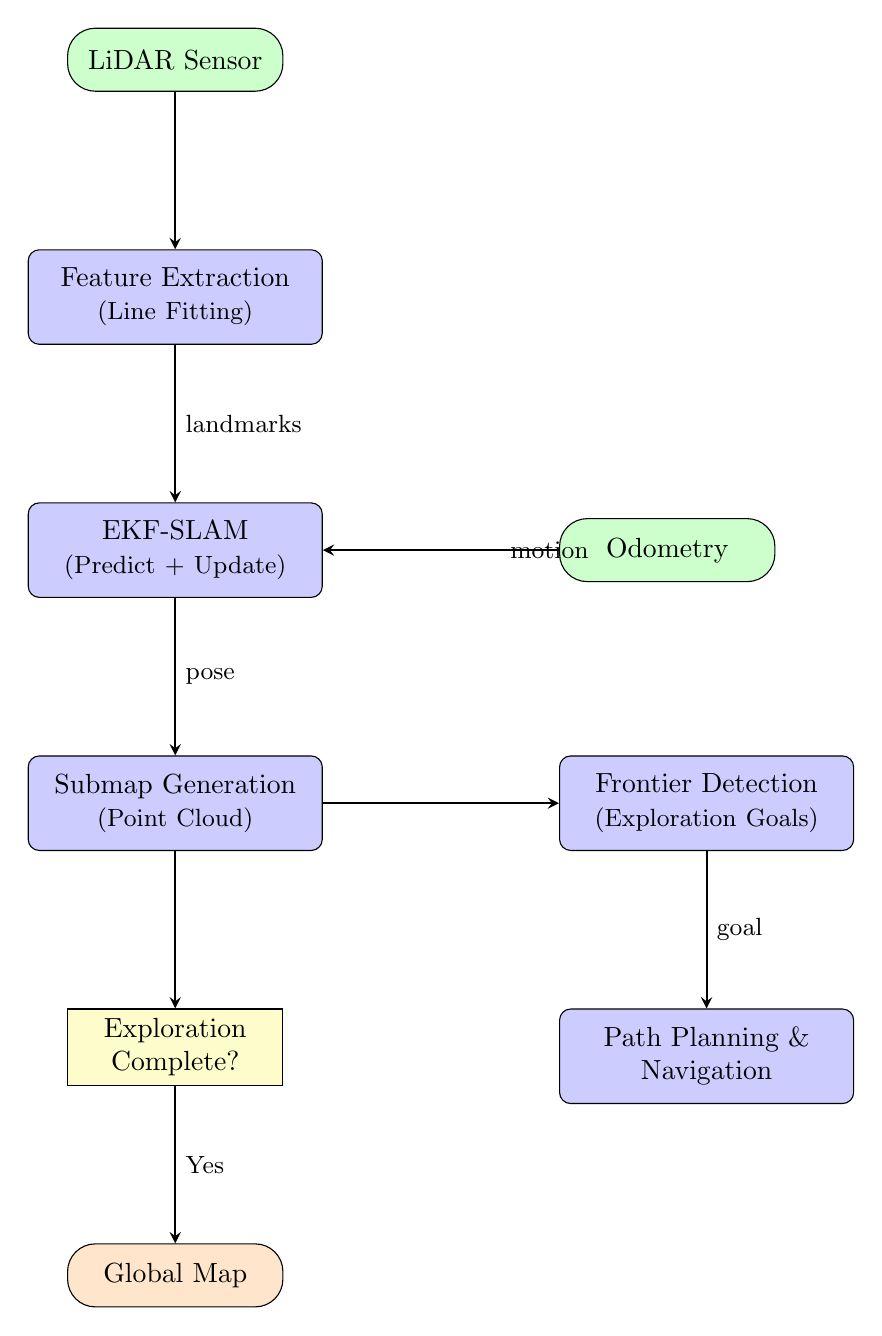
\begin{tikzpicture}[
		node distance=2cm and 3cm,
		block/.style={rectangle, draw, fill=blue!20, text width=3.5cm, align=center, minimum height=1.2cm, rounded corners},
		sensor/.style={rectangle, draw, fill=green!20, text width=2.5cm, align=center, minimum height=0.8cm, rounded corners=10pt},
		output/.style={rectangle, draw, fill=orange!20, text width=2.5cm, align=center, minimum height=0.8cm, rounded corners=10pt},
		decision/.style={rectangle, draw, fill=yellow!20, text width=2.5cm, align=center, minimum height=0.8cm},
		arrow/.style={->, >=stealth, thick},
		feedback/.style={->, >=stealth, thick, dashed, red}
		]
		
		% Sensors (top row)
		\node[sensor] (lidar) {LiDAR Sensor};
		
		% Processing blocks
		\node[block, below=of lidar] (feature) {Feature Extraction\\\small(Line Fitting)};
		\node[block, below=of feature] (slam) {EKF-SLAM\\\small(Predict + Update)};
		\node[block, below=of slam] (submap) {Submap Generation\\\small(Point Cloud)};
		
		\node[sensor, right=of slam] (odom) {Odometry};
		
		% Navigation branch
		\node[block, right=of submap] (frontier) {Frontier Detection\\\small(Exploration Goals)};
		\node[block, below=of frontier] (nav) {Path Planning \&\\Navigation};
		
		% Decision point
		\node[decision, below=of submap] (complete) {Exploration\\Complete?};
		
		% Outputs
		\node[output, below=of complete] (map) {Global Map};
		
		% Forward flow arrows
		\draw[arrow] (lidar) -- (feature);
		\draw[arrow] (odom) -- node[right, near start] {\small motion} (slam);
		\draw[arrow] (feature) -- node[right] {\small landmarks} (slam);
		\draw[arrow] (slam) -- node[right] {\small pose} (submap);
		\draw[arrow] (submap) -- (frontier);
		\draw[arrow] (frontier) -- node[right] {\small goal} (nav);
		\draw[arrow] (submap) -- (complete);
		\draw[arrow] (complete) -- node[right] {\small Yes} (map);
		
		
	\end{tikzpicture}
	\caption{High-level system architecture showing the main processing modules and flow of data from scan to final global map.}
	\label{fig:system_architecture}
\end{figure}

\subsection{Parameter Configuration}
\label{sec:parameter_configuration}

The system's performance depends critically on proper parameter tuning. This section details all key parameters used in the algorithm.

\subsubsection{Feature Extraction Parameters}

\begin{table}[htbp]
	\centering
	\caption{LiDAR and feature extraction parameters}
	\label{tab:lidar_params}
	\begin{tabular}{lcp{8cm}}
		\toprule
		\textbf{Parameter} & \textbf{Value} & \textbf{Rationale} \\
		\midrule
		\texttt{grow\_residual\_threshold} & 0.05 m & Maximum point-to-line residual during incremental line fitting \\
		\texttt{merge\_angle\_tolerance} & 0.35 rad & Maximum angle difference (20°) for merging adjacent parallel lines \\
		\texttt{merge\_rho\_tolerance} & 0.15 m & Maximum perpendicular distance for merging parallel lines \\
		\texttt{min\_line\_points} & 10 & Minimum points to form a reliable wall segment \\
		\texttt{min\_line\_length} & 0.5 m & Reject short segments that may be noise or small objects \\
		\texttt{max\_line\_gap} & 0.5 m & Maximum gap to merge adjacent collinear segments \\
		\texttt{corner\_angle\_threshold} & 45 & Minimum Angle between two intersecting lines to be considered as a corner\\
		\texttt{lidar\_noise\_sigma} & 0.01 m & LiDAR measurement standard deviation used for feature covariance computation \\
		\bottomrule
	\end{tabular}
\end{table}

All design parameters are chosen conservatively to reduce the risk of missing true features. For ranges of 1–3.5 m, a 1° scan yields roughly 3.5–6 cm lateral spacing; thus a 5 cm grow\_residual\_threshold accommodates lidar noise and range quantization while still rejecting clear outliers. A 45° corner threshold avoids labeling gentle bends or noisy segments as corners, which is conservative but appropriate in the maze environment where corners are predominantly 90°. Minimum line length and minimum line points provide an additional gate to prevent over‑segmentation of a single wall into multiple short segments.

\subsubsection{EKF-SLAM Parameters}

\begin{table}[htbp]
	\centering
	\caption{EKF-SLAM and association parameters}
	\label{tab:ekf_params}
	\begin{tabular}{lcp{8cm}}
		\toprule
		\textbf{Parameter} & \textbf{Value} & \textbf{Rationale} \\
		\midrule
		\texttt{chi\_sq\_gate} & 5.99 & 95\% confidence threshold ($\chi^2_{2,0.05}$) for 2-DOF \\
		\texttt{min\_observations\_for\_init} & 2 & Minimum observations before landmark initialization \\
		\texttt{wall\_angle\_tolerance} & 0.349 rad &  tolerance for parallel wall matching \\
		\texttt{wall\_rho\_tolerance} & 0.5 m & Distance tolerance for wall matching \\
		\texttt{max\_gap\_ext} & 1.0 m & Minimum gap between collinear walls to be associated as different wall landmarks. \\
		\bottomrule
	\end{tabular}
\end{table}

The chi-square gate threshold of 5.99 corresponds to the 95\% confidence level for a 2-DOF $\chi^2$ distribution, providing robust data association. Wall features additionally use geometric constraints: parallel walls must have angles within 20° and perpendicular distances within 0.5m for matching. The values are chosen a bit conservatively after trial and error method.

\subsubsection{Submap Generation Parameters}

\begin{table}[htbp]
	\centering
	\caption{Submap generation and stitching parameters}
	\label{tab:submap_params}
	\begin{tabular}{lcp{8cm}}
		\toprule
		\textbf{Parameter} & \textbf{Value} & \textbf{Rationale} \\
		\midrule
		\texttt{scans\_per\_submap} & 50 & Balance between local consistency and global coverage \\
		\texttt{voxel\_size} & 0.05 m & Downsampling resolution matching feature precision \\
		\texttt{icp\_max\_corr\_dist} & 0.05 m & Max distance for point correspondences; limits matches to nearby points \\
		\texttt{icp\_max\_iter} & 50 & Upper bound on ICP iterations before stopping \\
		\texttt{icp\_min\_fitness} & 0.3 & Reject alignment if too few inliers match \\
		\texttt{icp\_max\_rmse} & 0.05 m & Reject alignment if inlier error is too high \\		
		\bottomrule
	\end{tabular}
\end{table}

Using 50 scans per submap balances local consistency against accumulated drift, it yields enough points to stabilize feature estimates while keeping each submap short enough that odometry error does not dominate. A 0.05 m voxel size provides effective downsampling to reduce memory and computation while preserving wall geometry. Odometry drift is estimated using ground truth and odom values and accordingly the ICP correspondence gate is set to 0.05 m. This threshold limits nearest-neighbor pairings to points that are plausibly overlapping, rejecting distant matches and reducing outlier correspondences during submap alignment. The ICP minimum fitness threshold is intentionally lenient so alignments are not rejected when overlap is limited, while still filtering out extremely poor matches.

\subsubsection{Navigation and Exploration Parameters}

\begin{table}[htbp]
	\centering
	\caption{Navigation and exploration tuning parameters}
	\label{tab:navigation_params}
	\begin{tabular}{l c p{7.5cm}}
		\toprule
		\textbf{Parameter} & \textbf{Value} & \textbf{Description} \\
		\midrule
		\multicolumn{3}{l}{\textbf{SimpleNavigation (State Machine \& Reactive Avoidance)}} \\
		\texttt{scan\_emergency\_distance} & 0.5 m & Obstacle distance threshold for emergency slowing/replan \\
		\texttt{scan\_angular\_range} & 60$^\circ$ & Angular sector for obstacle checks \\
		\texttt{path\_deviation\_threshold} & 1.0 m & Replan if robot strays beyond this distance from path \\
		\texttt{stuck\_check\_window} & 5.0 s & Time window for stuck detection \\
		\texttt{stuck\_distance\_threshold} & 0.1 m & Minimum movement required in window \\
		\texttt{stuck\_timeout} & 30.0 s & Global timeout for EXECUTE\_PATH \\
		\midrule
		\multicolumn{3}{l}{\textbf{ConvexFrontierDetector (Frontier Detection)}} \\
		\texttt{frontier\_spacing} & 0.5 m & Boundary sampling spacing \\
		\texttt{boundary\_offset} & 0.5 m & Inward offset for safe frontier placement \\
		\texttt{candidate\_clearance} & 0.5 m & Reject candidate if too close to obstacle \\
		\texttt{score\_w\_travel} & 0.60 & Weight for travel distance score \\
		\texttt{score\_w\_heading} & 0.15 & Weight for heading alignment score \\
		\texttt{score\_w\_size} & 0.25 & Weight for directional cluster size score \\
		\midrule
		\multicolumn{3}{l}{\textbf{RRTStar (Path Planning)}} \\
		\texttt{safety\_margin} & 0.5 m & Collision clearance distance \\
		\texttt{step\_size} & 0.2 m & Tree extension step length \\
		\texttt{goal\_bias} & 0.5 & Probability of sampling the goal \\
		\texttt{max\_iterations} & 1500 & Maximum planning iterations \\
		\midrule
		\multicolumn{3}{l}{\textbf{PurePursuit (Path Tracking)}} \\
		\texttt{max\_linear\_velocity} & 0.20 m/s & Maximum forward speed \\
		\texttt{max\_angular\_velocity} & 1.0 rad/s & Maximum turning rate \\
		\texttt{lookahead} & 0.8 m & Lookahead distance \\
		\texttt{goal\_tolerance} & 0.3 m & Distance to consider goal reached \\
		\texttt{velocity\_gain} & 0.5 & Speed reduction on sharp turns \\
		\bottomrule
	\end{tabular}
\end{table}

The navigation parameters were tuned through multiple iterations of trial-and-error. Safety critical thresholds like scan\_emergency\_distance, safety\_margin, candidate\_clearance, and boundary\_offset are set to 0.5 m, a conservative multiple of the robot footprint to provide consistent clearance. In frontier scoring, the travel-cost term is weighted highest (0.60), followed by the size/information term (0.25), and then the heading term (0.15), to discourage oscillations between nearby frontiers. A 0.8 m lookahead distance balances responsiveness to upcoming turns with forward progress and obstacle avoidance. The RRT* planner is allowed up to 1500 iterations to trade off path quality against runtime and memory

\subsection{Qualitative Results}
\label{sec:qualitative_results}

In this work, only a small section of the maze environment has been mapped, and all plots are generated from data collected within that mapped region. The autonomous navigation module is not yet production‑grade and does not reliably handle extreme or edge‑case configurations. Despite these limitations, the data gathered is sufficient to evaluate the feature‑based SLAM algorithm, which explicitly models observation uncertainty during feature matching and localization.
\subparagraph{Raw Lidar scan and feature extraction}

\begin{figure}[htbp]
	\centering
	\includegraphics[width=0.5\textwidth]{../thesis_ws/images/landmarks.png}
	\caption{The figure illustrates how raw scan points are grouped into geometric landmarks.}
	\label{fig:feature_detection}
\end{figure}

The raw LiDAR scan is first split into segments wherever there is a gap between points. Each segment is then processed with incremental line fitting to extract wall candidates, shown as blue points. Intersections between adjacent wall segments form corners, shown as red points, as illustrated in Figure 4.


\begin{figure}[htbp]
	\centering
	\includegraphics[width=0.5\textwidth]{../thesis_ws/images/local_submap.png}
	\caption{Current local submap showing extracted features accumulated over multiple LiDAR scans.}
	\label{fig:local_submap}
\end{figure}

\subparagraph{Local Submap} 

The local submap view shown in figure 5 depicts the submap built from a short window of recent scans, where each feature is rendered as a point cloud by interpolating points between its endpoints.

\subparagraph{Global Map}
The map shown in Figure 6 uses white point clouds to depict the final stitched global map. The blue boundary is the convex hull, which marks the frontier between explored and unexplored regions. Multiple frontiers are shown as red and orange spheres; the red sphere indicates the active frontier goal, which is rated using travel cost, information cost, and heading cost

\begin{figure}[htbp]
	\centering
	\includegraphics[width=0.5\textwidth]{../thesis_ws/images/map_4.png}
	\caption{Convex hull boundary (white/blue polygon) computed from the current map points. The hull defines the boundary between explored and unexplored regions, with the robot shown at the lower-left corner.}
	\label{fig:convex_hull}
\end{figure}

% ==============================================================================
\subsection{Results}
\label{sec:quantitative_results}

\subsubsection{Comparison between Robot estimated Pose and Ground Truth}

The EKF vs. ground‑truth plot shows close agreement over the full trajectory, indicating that the filter tracks the true motion well. A small, consistent offset appears in the middle segment, which is consistent with a feature‑sparse corridor: the robot can constrain its position perpendicular to the wall but remains uncertain along the wall direction. There is no catastrophic divergence, and overall the EKF remains stable relative to ground truth.

\subparagraph{Abosulte Trajectory Error}
Absolute Trajectory Error (ATE) measures the deviation between the estimated trajectory and ground truth. It is typically summarized using the root mean square error (RMSE), which provides a single scalar for overall trajectory accuracy; lower RMSE indicates closer agreement. For the collected data, the RMSE is 0.14 m, corresponding to an average positional error of about 14 cm between the EKF estimate and ground truth.

\begin{figure}[htbp]
	\centering
	\includegraphics[width=0.75\textwidth]{../thesis_ws/images/ekf_vs_groundtruth.png}
	\caption{Comparison between Ekf trajectory and actual ground truth from the simulation.}
	\label{fig:ATE}
\end{figure}

\subsubsection{Uncertainity in robot Pose}
\begin{figure}[htbp]
	\centering
	\includegraphics[width=0.75\textwidth]{../thesis_ws/images/uncertainity_in_robot_position.png}
	\caption{EKF position covariance across submaps, showing variance in the x and y directions}
	\label{fig:Variance}
\end{figure}
The uncertainty plot shown in figure$~$\ref{fig:Variance} shows the EKF’s positional variance in x and y direction across submaps. Periods where the variance is strongly anisotropic (one axis higher than the other) indicate directional ambiguity: the filter is well‑constrained perpendicular to the corridor wall direction but less certain along the corridor axis. This supports the earlier interpretation that the small mid‑segment offset arises from feature‑sparse corridor geometry, which provides limited constraints in the along‑wall direction.

\subsubsection{Submap Confidence Evolution}

\begin{figure}[htbp]
	\centering
	\includegraphics[width=0.75\textwidth]{../thesis_ws/images/submap_confidence_2.png}
	\caption{Confidence value for each submap generated}
	\label{fig:submap_confidence}
\end{figure}

The confidence metric is computed as:
\begin{equation}
	C(t) = 1 - \exp\left(-\frac{I_{\text{landmarks}}(t)}{\tau}\right)
\end{equation}
where $I_{\text{landmarks}}$ is the sum of landmark information (trace of inverse variance) and $\tau = 10^6$ is a normalization constant.

The submap‑confidence plot in Figure~\ref{fig:submap_confidence} shows how the EKF confidence metric evolves across submaps. It begins near zero for the first submap, then rises quickly and stabilizes around 0.8–1.0 as more reliable landmarks are incorporated. The initial dip around submap 3 to 8 correspond to the long corridor section, which yields fewer informative features and lowers the summed information. Overall, the trend indicates that the estimator reaches and sustains high confidence once the environment becomes feature‑rich in all directions.

\section{Conclusion and Future Works}

This thesis presents a comprehensive feature-based EKF-SLAM system for autonomous indoor exploration that addresses the fundamental challenge of probabilistic mapping and localization in GPS-denied environments. The work demonstrates rigorous uncertainty modeling, and using it for sensor fusion. It also presents a frontier based navigation algorithm for a point cloud based map using convex hull to differentiate between explored and unexplored reigon.

Unlike many feature-based approaches that rely on heuristic covariance assignments, this system derives landmark uncertainties. Wall covariances are computed using the Fisher Information Matrix (Cramér-Rao Lower Bound). Corner covariances are propagated analytically through the line intersection geometry using the Jacobian of the transformation. 

Walls are represented using Hessian parameters $(\rho, \alpha)$ which provides a compact two-degree-of-freedom representation that is free from singularities encountered in slope-intercept forms. The parametric extent tracking $(t_{\text{min}}, t_{\text{max}})$ allows wall segments to grow dynamically as new observations arrive, preventing over segmentation while maintaining geometric consistency.

The submap stitching module employs point-to-point ICP alignment with uncertainty quantification. By extracting point correspondences and building the Fisher Information Matrix from the alignment Jacobian, the system produces a 3×3 pose correction covariance that captures the quality of the alignment. The navigation module introduces a grid-free frontier detection strategy that operates directly on the point cloud map. By computing the convex hull of observed free space and sampling along the buffered boundary, the system generates exploration targets without the discretization used in occupancy grid methods.

\subparagraph{Future Work}

In this work, there are a lot of areas which can be improved to obtain a more robust algorithm for feature based SLAM.

One of them would be to improve the covariance estimates of the feature extracted and ICP based submap stiching by including more sources of error. Another improvement to the system, would be to find a better way to evaluate corresponding pairs for ICP than using nearest point within a threshold.

The current 2D planar assumption limits applicability to environments with stairs, ramps, or multi-level structures. The current system can be extended to 3D mapping, extracting features in 3D space, and augmenting the EKF state to include pitch and roll. This would enable operation in parking garages, stairwells, and outdoor terrains.

Real-world indoor spaces frequently contain moving objects such as people, doors, and furniture. Future work could incorporate dynamic object detection. Static landmarks could be distinguished from dynamic objects using consistency checks over multiple observations, allowing the EKF to maintain only persistent features while tracking dynamic obstacles separately for collision avoidance.

While the EKF provides real-time estimates, it suffers from linearization errors and computational scaling with map size. Transitioning to a graph-based backend using pose graphs and factor graphs (e.g., GTSAM or g2o) would enable batch optimization of the full trajectory and all landmarks. Loop closure constraints could be added as factors, and the graph could be optimized periodically using Levenberg-Marquardt or Gauss-Newton methods. This would reduce accumulated drift and improve global consistency, especially for large-scale exploration.

The current system relies on hand-tuned parameters for feature extraction, data association, and navigation. Future work could incorporate adaptive or learning-based parameter adjustment. Submap confidence metric can be used to determine the next frontier by reexploring sections with low confidence values.

These future works collectively represent a roadmap toward a fully autonomous, robust, and scalable SLAM system capable of operating in diverse real-world environments.


\begin{thebibliography}{9}
	
	
	\bibitem{smith1987}
	R.~C. Smith and P. Cheeseman, 
	``On the representation and estimation of spatial uncertainty,'' 
	\emph{The International Journal of Robotics Research}, 
	vol.~5, no.~4, pp. 56--68, 1987.
	
	\bibitem{durrant2006slam}
	H.~Durrant-Whyte and T.~Bailey,
	``Simultaneous localisation and mapping (SLAM): Part I the essential algorithms,''
	\emph{IEEE Robotics \& Automation Magazine},
	vol.~13, no.~2, pp.~99--110, 2006.
	
	\bibitem{Shuien2020}
	Shuien Yu, Chunyun Fu, Amirali K. Gostar and Minghui Hu,
	``A Review on Map-Merging Methods for Typical Map Types in Multiple-Ground-Robot SLAM Solutions,''
	\emph{Sensors}, vol. 20, p. 6988, 
	2020. doi:10.3390/s20236988.
	
	\bibitem{Dissanayake2001}
	G. Dissanayake, P. Newman, S. Clark, H. F. Durrant-Whyte and M. Csorba, 
	``A solution to the simultaneous localisation and map building (SLAM) problem,'' 
	\emph{IEEE Transactions on Robotics and Automation}, vol. 17, no. 3, 
	June 2001.
	
	\bibitem{kim2018scan}
	G.~Kim and A.~Kim,
	``Scan context: Egocentric spatial descriptor for place recognition within 3D point cloud map,''
	\emph{2018 IEEE/RSJ International Conference on Intelligent Robots and Systems (IROS)},
	pp.~4802--4809, 2018.
	
	\bibitem{Nguyen}
	Nguyen V., Martinelli, A., Tomatis, N., \& Siegwart, R.
	``A Comparison of Line Extraction Algorithms using 2D Laser Rangefinder for Indoor Mobile Robotics.``
	\emph{Proceedings of IEEE/RSJ IROS}
	pp. 1929–1934.
	
	\bibitem{grisetti2010graph}
	G.~Grisetti, R.~K{\"u}mmerle, C.~Stachniss, and W.~Burgard,
	``A tutorial on graph-based SLAM,''
	\emph{IEEE Intelligent Transportation Systems Magazine},
	vol.~2, no.~4, pp.~31--43, 2010.
	
	\bibitem{Yamauchi1997}
	Yamauchi, B.,
	``A frontier-based approach for autonomous exploration``,
	\emph{Proceedings 1997 IEEE International Symposium on Computational Intelligence in Robotics and Automation CIRA'97. 'Towards New Computational Principles for Robotics and Automation},
	pp.~ 146-151, DOI 10.1109/CIRA.1997.613851, 1997
	
	
	\bibitem{karaman2011sampling}
	S.~Karaman and E.~Frazzoli, 
	``Sampling-based algorithms for optimal motion planning,''
	\emph{The International Journal of Robotics Research}, 
	vol.~30, no.~7, pp.~846--894, 2011.
	
	\bibitem{barber1996quickhull}
	C.~B.~Barber, D.~P.~Dobkin, and H.~Huhdanpaa,
	``The quickhull algorithm for convex hulls,''
	\emph{ACM Transactions on Mathematical Software (TOMS)},
	vol.~22, no.~4, pp.~469--483, 1996.
	
	\bibitem{coulter1992}
	R. C. Coulter,
	``Implementation of the Pure Pursuit Path Tracking Algorithm,''
	\textit{Technical Report CMU-RI-TR-92-01},
	Robotics Institute, Carnegie Mellon University, 1992.
	
	\bibitem{ekf_practice}
	Alaa Aldeen Housein, Gao Xingyu*, Weiming Li, Yang Huang,
	``Extended Kalman filter sensor fusion in practice for mobile robot localization,''
	\emph{(IJACSA) International Journal of Advanced Computer Science and Applications},
	Vol. 13, No. 2, 2022.
	
	\bibitem{lidar_imu_wheel}
	Shaojiang Zhang, Yanning Guo
	, Qiang Zhu , Zhiyuan Liu ,
	``LiDAR-IMU and wheel odometer based autonomous vehicle localization system,''
	\emph{The 31th Chinese Control and Decision Conference },
	2019.
	
	\bibitem{visual_slam}
	[Takafumi Taketomi, Hideaki Uchiyama and Sei Ikeda],
	``Visual SLAM algorithms: a survey from
	2010 to 2016,''
	\emph{IPSJ Transactions on Computer Vision and
		Applications},
	(2017) 9:16
	DOI 10.1186/s41074-017-0027-2.
		
	\bibitem{burgard2000collaborative}
	W.~Burgard, M.~Moors, C.~Stachniss, and F.~E.~Schneider,
	``Collaborative multi-robot exploration,''
	\emph{Proceedings 2000 ICRA. Millennium Conference. IEEE International Conference on Robotics and Automation},
	vol.~1, pp.~476--481, 2000.
	
	\bibitem{lajoie2024swarm}
	P.-Y.~Lajoie and G.~Beltrame,
	``SWARM-SLAM: Sparse decentralized collaborative simultaneous localization and mapping framework for multi-robot systems,''
	\emph{IEEE Robotics and Automation Letters},
	vol.~9, no.~1, pp.~475--482, 2024.
	
	\bibitem{pomerleau2015icp}
	F.~Pomerleau, F.~Colas, and R.~Siegwart,
	``A review of point cloud registration algorithms for mobile robotics,''
	\emph{Foundations and Trends in Robotics},
	vol.~4, no.~1, pp.~1--104, 2015.
	
	\bibitem{rep105}
	REP 105: Coordinate Frames for Mobile Platforms. 
	\url{https://www.ros.org/reps/rep-0105.html}
	
	\bibitem{zhou2018open3d}
	Q.-Y. Zhou, J. Park, and V. Koltun,
	``Open3D: A Modern Library for 3D Data Processing,''
	\textit{arXiv:1801.09847}, 2018.
	
	\bibitem{dellaert2012gtsam}
	F. Dellaert,
	``Factor Graphs and GTSAM: A Hands-on Introduction,''
	Technical Report GT-RIM-CP\&R-2012-002, Georgia Institute of Technology, 2012.
	
	\bibitem{thrun2005probabilistic}
	Thrun, Sebastian and Burgard, Wolfram and Fox, Dieter,
		"Probabilistic Robotics",
		2005, MIT Press
	
	
	
\end{thebibliography}


\end{document}